\documentclass[preprint,11pt,authoryear]{elsarticle}
\usepackage{amsmath,amssymb,amsthm,bm}
\usepackage{graphicx,booktabs,multirow,xcolor}
\usepackage[hidelinks]{hyperref}
\usepackage{siunitx}
\usepackage{microtype}
\emergencystretch=2em
\sisetup{group-separator={,},group-minimum-digits=4}
\newtheorem{proposition}{Proposition}
\newcommand{\lta}{\textsc{LTA}}
\journal{International Journal of Forecasting}

\begin{document}
\begin{frontmatter}
\title{Where leading covariates are lost in frozen time-series foundation models: horizon alignment versus adaptation in a pre-registered study of rivers, weather, wind power and traffic}

\author[1]{Author One}
\author[1]{Author Two}
\address[1]{Affiliation (to be completed)}

\begin{abstract}
Time-series foundation models (TSFMs) are known to make poor use of covariates. We locate where this happens for covariates that are observed only in the past and lead the target: their information is recovered only when it reaches the forecast horizon. In a pre-registered synthetic test, shifting the covariate forward by its true lead lowered MASE by 31--39\% for Chronos-2, TimesFM-2.5 and TabPFN-TS, whereas shifting only the context, or by a random lag, did not. The Lead-Time Aligner (\lta{}), a 21k-parameter module trained once on synthetic data through the frozen Chronos-2, beat cross-correlation shifting by 7.7--9.7\% where lags vary with system state or responses are distributed, and transferred without retraining to the other two backbones. On four new pre-registered benchmarks with random-lag controls, we compare zero-shot alignment with a trained frozen-backbone adapter (CoRA), supervised ARX and LightGBM, and fine-tuning. On nine river pairs, zero-shot \lta{} lowered Chronos-2 error by 14.5\% relative to no covariate, more than CoRA or supervised models trained on six years of data; only fine-tuning was better. Its margin over classical alignment was small and seed-dependent. For wind generation and air pressure the relation was essentially simultaneous, and alignment gains were absent or not lead-specific. For road traffic the lead was long but weak, and nothing beat the raw covariate. For TimesFM-2.5, TabPFN-TS and Moirai-1.1, a raw past-only river covariate was harmful (13--33\%). In our benchmarks alignment paid off only where the lead was both multi-step and strong, which a training-split diagnostic can check.
\end{abstract}

\begin{keyword}
time-series foundation models \sep covariates \sep lead--lag \sep time-delay estimation \sep zero-shot forecasting \sep adapters \sep hydrology \sep wind power \sep traffic \sep pre-registration
\end{keyword}
\end{frontmatter}

%======================================================================
\section{Introduction}
\label{sec:intro}

Pretrained time-series foundation models (TSFMs) forecast unseen series zero-shot and, since 2025, accept covariates: Chronos-2 attends across a group of target and covariate series \citep{ansari2025chronos2}, TimesFM-2.5 regresses its residual on covariates in context \citep{das2024timesfm,timesfm_github}, and TabPFN-TS casts forecasting as tabular regression over time-indexed features \citep{hoo2025tabpfnts}. Many practically important covariates are \emph{leading indicators}: they are observed only up to the forecast origin, but they affect the target after a physical delay. Upstream discharge reaches a downstream gauge after a flow-dependent travel time; a pressure system reaches a downwind city after an advection time set by the wind. For such covariates the information needed for the first part of the forecast horizon has already been observed.

Recent diagnostic work shows that TSFMs exploit such covariates poorly. On SimpleTimeBench, where the past covariate is an exact copy of the target shifted 48 steps ahead, Chronos-2 improves only marginally on random walks (relative MAE 1.02 to 0.98). On an upstream--downstream river pair, the covariate lowers MASE by 5.9\% for Chronos-2 against 24.2\% for an 840-parameter DLinear \citep{ghoroghchian2026foundations}. \citet{won2026attenuated} find that in-context identification of forced systems is attenuated in Chronos-2, and that the predictions of TimesFM-2.5 and TabPFN-TS respond almost only to same-time covariate values. Appending 32 lagged copies of a \emph{known} input restores their sensitivity, which led that author to conclude that the covariate interface, rather than the backbone, is the limit. These studies repair the failure by fine-tuning, which degrades univariate accuracy, or by fixed lag banks. They do not address \emph{past-only} leading covariates, whose values are missing over the horizon, nor do they offer an estimated alignment that leaves the pretrained model untouched.

We build on these diagnoses rather than repeat them. Our question is narrower and practical: for a covariate that is observed only in the past and leads the target, \emph{where} in the forecasting pipeline is its information lost, and what is the best way to recover it when the backbone must stay frozen? This paper makes four contributions.

\textbf{(i) A mechanism test that locates the loss at the horizon.} Extending the interface argument of \citet{won2026attenuated} from known inputs to past-only covariates, we show that for three covariate-aware TSFMs with different covariate mechanisms, the information carried by a leading covariate is recovered only when its values are placed in the forecast horizon. Chronos-2 masks a past-only covariate over the horizon, and the regressions of TimesFM-2.5 (XReg) and TabPFN-TS couple only same-time values. In a pre-registered headroom test, re-indexing the covariate forward by its true lead lowered error by 31--39\%. The same shift applied to the context only, or a shift by a random lag, did not help, which isolates the horizon as the place where information is lost (Section~\ref{sec:gate}).

\textbf{(ii) A learned aligner that transfers across backbones.} The Lead-Time Aligner (\lta{}) estimates a static lead from cross-correlation evidence, adds a state-dependent offset, and moves covariate values to their arrival times by differentiable soft splatting (Section~\ref{sec:method}). It is trained once, on synthetic tasks only, through the frozen Chronos-2. On held-out synthetic tasks it beats classical delay estimation where leads vary with the system state or responses are distributed, and this advantage carries over without retraining to TimesFM-2.5 and TabPFN-TS.

\textbf{(iii) Four pre-registered real-world benchmarks with specificity controls.} RiverLead pairs nine upstream and downstream USGS gauges, AirLead ten upwind and downwind ERA5 pressure series, EnergyLead ten neighbouring wind-generation areas in Europe, and TrafficLead ten downstream and upstream freeway detectors in the San Francisco Bay Area. Hypotheses, arms, splits and pass rules were frozen before the forecasts were run, every deviation is reported (\ref{app:deviations}), and every aligned arm is tested against a random-lag control.

\textbf{(iv) A cross-backbone, cross-method account of the real-world trade-off.} We compare zero-shot alignment with six classical delay estimators, a trained frozen-backbone adapter (CoRA; \citealp{qin2025cora}), supervised ARX and LightGBM models trained on short and full histories, and full and LoRA fine-tuning of Chronos-2, on four backbones.

The results define when each tool is worth using. Where a physical lead of several hours exists (rivers), zero-shot alignment of a frozen Chronos-2 was more accurate overall than a CoRA adapter and than supervised models trained on six years of each river's history, although the strongest supervised model won three of nine rivers and flood-event windows; only fine-tuning the backbone was better overall. Where the shared signal is simultaneous (wind power), alignment had nothing to move into the horizon, and the trained adapter was the most useful frozen option. Where the lead is long but weak (road traffic), no method improved on the raw covariate. On weather, the gains from alignment with Chronos-2 were not specific to the lead. Across backbones, a raw past-only covariate made three of four TSFMs worse than no covariate on rivers, and alignment only partly repaired this. The learned aligner improved clearly on classical alignment on synthetic data and with TimesFM-2.5 on rivers, but with Chronos-2 its margin on real data was small and seed-dependent. We report these outcomes as they were obtained, including the hypotheses that were not supported.

%======================================================================
\section{Related work}
\label{sec:related}

\paragraph{Covariates in TSFMs} Chronos-2 alternates time attention with group attention over targets, past-only covariates and known covariates; in the horizon, entries of targets and past-only covariates are set to missing \citep{ansari2025chronos2}. TimesFM was proposed with in-context covariate regression on the forecast residual \citep{das2024timesfm}, implemented for TimesFM-2.5 as XReg \citep{timesfm_github}. TabPFN-TS regresses the target on time-indexed features and supports only covariates known in both history and horizon \citep{hoo2025tabpfnts,hollmann2025tabpfn}. Moirai flattens variates and time into one sequence and accepts dynamic covariates \citep{woo2024moirai}. Covariate-aware benchmarks include fev-bench \citep{shchur2025fevbench} and GIFT-Eval \citep{aksu2024gifteval}.

\paragraph{Adapting frozen TSFMs to covariates} ChronosX injects past covariates into token embeddings and future covariates into output logits of a frozen Chronos \citep{arango2025chronosx}. UniCA homogenises heterogeneous covariates and fuses them before and after a frozen encoder, with all covariates aligned at the same time index \citep{han2026unica}. CoRA reduces each covariate to its last-step embedding and modulates the frozen head with Granger-weighted features; its Granger lag is an offline diagnostic and is not used to re-index covariates \citep{qin2025cora}. Because it is the most recent adapter designed for exactly this setting, we use it as the trained frozen-backbone baseline (Section~\ref{sec:cross}). TFMAdapter refines frozen forecasts with a Gaussian process on same-time covariates \citep{dange2025tfmadapter}, and $\delta$-Adapter edits covariates additively or multiplicatively in front of a frozen forecaster without temporal re-indexing \citep{liang2026deltaadapter}. Parameter-generation and memory adapters do not use covariates \citep{nallagatla2026adacast,lyu2026tsmemory}. CITRAS-FM shifts \emph{known} covariates by a fixed one-patch offset inside cross-variate attention of a model trained for that purpose \citep{yamaguchi2026citrasfm,yamaguchi2026citras}. None of these estimates a covariate's lead time and re-indexes a past-only covariate into the horizon of a frozen model.

\paragraph{Leading indicators and delay estimation} Transfer-function and distributed-lag models make covariate delays explicit \citep{box1970,box2008,almon1965}, Granger causality formalises lead--lag predictability \citep{granger1969}, and generalised cross-correlation with phase transform (GCC-PHAT) is a standard time-delay estimator \citep{knapp1976}. LIFT is the closest method. It estimates a per-window integer lead by FFT cross-correlation and shifts the leading channels, filling any part of the horizon not covered by observed values with the backbone's own forecast of the leader. It then fuses the shifted leaders with the \emph{output} of the backbone in a trained frequency-domain refiner; the backbone, a dataset-specific supervised model, is trained jointly or frozen after in-domain training \citep{zhao2024lift}. DeltaLag learns attention-selected integer lags for next-day stock returns end to end \citep{zhou2025deltalag}, DeMa uses a cross-correlation delay as a rotary position offset inside attention \citep{an2026dema}, and SLA-DLinear adds a soft lag-attention adapter to a DLinear model for closed multivariate forecasting, with the backbone trained per dataset, fine-tuned jointly with the adapter, and the lag weights fixed at inference \citep{luo2026sladlinear}. LACMT selects one lag per exogenous channel on training data and builds the horizon context of a demand transformer trained from scratch by indexing each past covariate at $t+h-\ell$, clamped to the last observed value so that no future value leaks \citep{vale2026lacmt}; our TimesFM-2.5 input uses the same clamping rule (Section~\ref{sec:arms}). Supervised exogenous-variable architectures such as TimeXer, iTransformer, PatchTST and DLinear learn delays implicitly from in-domain data \citep{wang2024timexer,liu2024itransformer,nie2023patchtst,zeng2023dlinear}. Our setting differs in three respects: the forecaster is a pretrained foundation model used zero-shot; the shifted covariate enters the backbone's \emph{input} as a known covariate, so the backbone's own covariate mechanism consumes it; and the lead estimator is learned, state-dependent and amortised across tasks. A fixed, hand-chosen version of the input shift has been suggested informally for SimpleTimeBench \citep{jjakimoto2026issue1936}; we test it systematically and extend it to estimated and state-dependent leads.

\paragraph{Diagnostics of covariate use} SimpleTimeBench documents covariate underutilisation by TSFMs, including on the Delaware River pair that RiverLead extends \citep{ghoroghchian2026foundations}. \citet{won2026attenuated} show that appending 32 lagged copies of a known input raises the covariate sensitivity of TimesFM-2.5 and TabPFN-TS, and that fine-tuning Chronos-2 on synthetic forced systems repairs attenuation but worsens univariate M4-hourly MASE from 0.69 to 0.89. \citet{berthelier2026investigating} probe same-time target--covariate relations in Chronos-2 and TabPFN-TS.

%======================================================================
\section{Where leading information is lost}
\label{sec:interface}

Let $y_{1:C}$ be the target context, $H$ the horizon, and $x_{1:C}$ a past-only covariate with lead $\tau_t\ge 0$, meaning that $y_t$ depends on $x_{t-\tau_t}$ (possibly through a kernel over several lags). A TSFM with a covariate interface receives $(y_{1:C}, x_{1:C}, \tilde x_{C+1:C+H})$, where $\tilde x$ holds future covariate values and is entirely missing for a past-only covariate.

\paragraph{Chronos-2} Past-only covariates are represented over the horizon by missing values \citep{ansari2025chronos2}, so horizon tokens of the target can attend only to same-position covariate tokens that carry no value. Any use of $x$ for the forecast must pass through time attention inside the context, which our results show is weak (Section~\ref{sec:gate}).

\paragraph{TimesFM-2.5 (XReg) and TabPFN-TS} XReg fits $y_t - \hat y^{\mathrm{TSFM}}_t \approx \beta^\top \tilde x_t$ on the context and applies $\beta$ to the horizon; TabPFN-TS regresses $y_t$ on features observed at time $t$. Both couple only same-time values, and both require $\tilde x$ in the horizon \citep{won2026attenuated,hoo2025tabpfnts}.

\paragraph{Re-indexing} Define the aligned covariate $a_t = x_{t-\tau_t}$ on the target clock. Because $x$ is observed up to $C$, $a_t$ is observed for every horizon step with $t-\tau_t\le C$, i.e.\ for the first $\min(\tau,H)$ steps when $\tau$ is constant. Passing $a$ as a \emph{known} covariate (values where observed, missing elsewhere), together with the raw past covariate, puts the leading information exactly where each interface can use it: in the horizon, at the same index as the target value it explains.

\begin{proposition}\label{prop:same-time}
Suppose $y_t = \beta x_{t-\tau} + \varepsilon_t$ with $\varepsilon$ independent of $x$, $\tau\ge H$, and a forecaster whose horizon prediction is a same-time linear function $\hat y_t = \gamma^\top z_t$ of the covariate vector $z_t$ supplied at time $t$. If $z_t = x_t$ (raw covariate, unavailable for $t>C$) the covariate cannot reduce horizon error. If $z_t = a_t = x_{t-\tau}$, which is observed for all $t\le C+H$, the least-squares $\gamma$ fitted on the context is a consistent estimator of $\beta$ as $C\to\infty$, and the expected squared horizon error converges to the noise variance.
\end{proposition}
The proof follows from standard least-squares consistency, since $a_t$ and $\varepsilon_t$ are independent. The proposition explains the mechanism we test empirically: re-indexing \emph{and} providing the re-indexed values in the horizon are both necessary. Re-indexing only the context leaves the horizon empty, which is why our ``context-only'' control is uninformative.

%======================================================================
\section{The Lead-Time Aligner}
\label{sec:method}

\lta{} maps $(y_{1:C}, x_{1:C})$ to an aligned covariate $a_{1:C+H}$ with missing entries wherever the source value is not observed. The backbone then receives the raw past covariate $x$ and the aligned covariate $a$, the latter as a known covariate. Because the raw covariate is always kept, alignment can only add information. Figure~\ref{fig:arch} summarises the module; it has \num{21284} parameters.

\paragraph{Lag evidence} On the context we compute five normalised cross-correlation profiles $r^{(j)}(\ell)=\mathrm{corr}(y_t, x_{t-\ell})$, $\ell=0,\dots,K$ with $K=168$, by FFT: on raw values, first differences, AR(1)-prewhitened series, absolute differences and ranks. These cover linear, trending, autocorrelated, magnitude-driven and monotone-nonlinear relations.

\paragraph{Static lead} A three-layer dilated 1-D CNN over the lag axis (width 32, kernel 7, dilations 1, 2, 4) reads the five profiles and a position channel and outputs a residual on top of the classical estimate,
\begin{equation}
\psi(\ell) = \kappa\,\bigl|r^{(1)}(\ell)\bigr| + \mathrm{CNN}(r^{(1:5)})_\ell,
\end{equation}
where $\kappa$ is learnable (initialised at 10) and the CNN output layer is zero-initialised, so that training starts from cross-correlation alignment. Mean- and max-pooled CNN features give an instance embedding $e\in\mathbb{R}^{32}$ and a temperature $T=\mathrm{softplus}(w^\top e)+0.05$.

\paragraph{State-dependent offset} For each source time $s$ the lead is perturbed by $\delta_s = D\tanh\bigl(g([\phi_s, e])\bigr)$ with $D=24$, where $\phi_s$ contains the standardised covariate, two causal exponential moving averages (0.9, 0.98), its first difference and its log-level relative to the context median, and $g$ is a three-layer MLP with zero-initialised output. This lets the lead shorten at high flow or strong wind, as travel-time physics suggests.

\paragraph{Soft forward splatting} Every source value $x_s$ is assigned to target times by a softmax over sources,
\begin{equation}
w_{t,s} = \operatorname{softmax}_s\!\Bigl(\psi\bigl(t-s-\delta_s\bigr)/T\Bigr),\qquad 0\le t-s-\delta_s\le K,
\end{equation}
with linear interpolation of $\psi(\cdot)$ between integer lags. The source axis includes $K$ unobserved positions before the context and the $H$ unobserved horizon positions, so probability mass on unobserved sources is accounted for rather than renormalised away. The aligned value is $a_t = \sum_{s\le C} w_{t,s} x_s / \pi_t$ with observed share $\pi_t=\sum_{s\le C} w_{t,s}$, and $a_t$ is declared missing when $\pi_t<\rho=0.5$. With a one-hot $\psi$, zero offsets and a small temperature, the operator reproduces the integer shift exactly, including its missingness pattern; we verified this with a unit test.

\paragraph{Training through a frozen backbone} Chronos-2 is differentiable with explicit context and covariate masks, so we train \lta{} end to end with the backbone frozen. The forecasting loss is the Chronos-2 quantile loss over its 21 quantile levels, scaled per series by the in-sample seasonal-naive MAE ($m=24$). Two auxiliary losses, active only for synthetic families with a point lead, are a cross-entropy between the softmax of $\psi/T$ and the median true lag, and the scaled squared error between $a$ and the oracle-aligned covariate. Without them the zero-initialised layers receive no gradient at the start of training. We train on a fixed pool of \num{30000} synthetic tasks (Section~\ref{sec:data}) with AdamW (learning rate $2\times10^{-3}$, weight decay $10^{-4}$, batch 32, gradient clipping 1.0) for 3,000 steps and keep the checkpoint with the best validation GM-MASE on 400 held-out synthetic tasks, evaluated every 250 steps (selected steps: 1,500, 2,750 and 1,500 for seeds 0--2). Training takes about 35 minutes on one NVIDIA T4, including validation.

\paragraph{Transfer} The trained aligner is backbone-agnostic at inference: its output is a covariate series. We pass the same aligned covariates to TimesFM-2.5 (XReg, fitted per series), TabPFN-TS and Moirai-1.1 without retraining.

\begin{figure}[t]
\centering
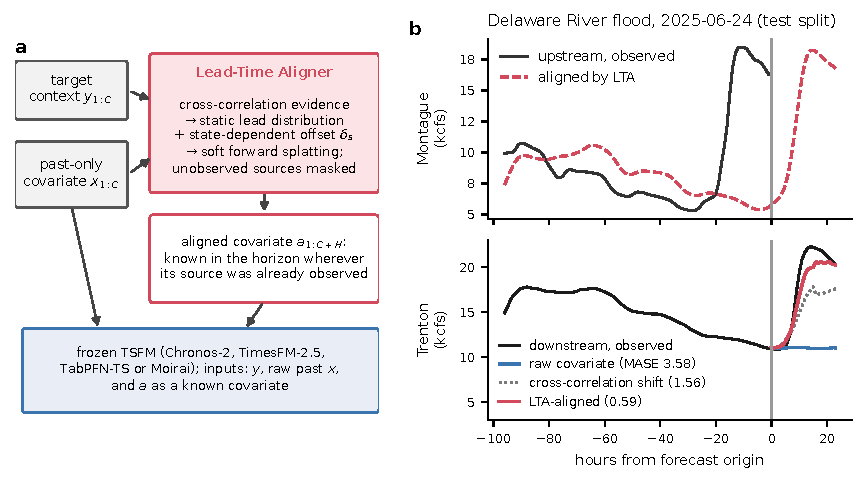
\includegraphics[width=\linewidth]{figs/fig0_arch.pdf}
\caption{Lead-Time Aligner. Five cross-correlation profiles give a static lead distribution (residual on classical cross-correlation); a state-dependent offset adjusts the lead of each source time; soft forward splatting moves covariate values to their arrival times and marks arrivals from unobserved sources as missing. The frozen TSFM receives the raw past covariate and the aligned covariate as a known covariate. (b) A Delaware River flood in the RiverLead test period: upstream discharge at Montague and its \lta{}-aligned version (top), and Chronos-2 forecasts at Trenton with the raw covariate, the top-3 cross-correlation shift and the \lta{}-aligned covariate (bottom), with per-window MASE in parentheses.}
\label{fig:arch}
\end{figure}

%======================================================================
\section{Experimental design}
\label{sec:data}

\subsection{Pre-registration}
Six protocols were frozen before the forecasts they govern were run: the headroom gate (P0), RiverLead (P2), ablations and seeds (P3), AirLead (P4), a revision protocol (P5) covering synthetic transfer, EnergyLead, supervised lagged baselines and a frozen-adapter baseline, written after an internal review of the first four, and TrafficLead (P6). Each lists what had been observed at freezing time, the arms, metrics, tests and pass rules. Deviations are logged with their cause and consequence in \ref{app:deviations}; none changed a hypothesis or a pass rule.

\subsection{LeadBench-S: synthetic leading-indicator tasks}
Each task is simulated on a long clock with a 400-step burn-in and cut to $C+H=512+24$ steps. Covariates are standardised AR(1) processes ($\phi\in[0.85,0.98]$) except in two families: \emph{periodic} (a 24-step seasonal pattern plus AR(1) noise) and \emph{pulse} (sparse exponential pulses, rate 2--5\%). The target is $y_t=\mu+\beta\, d_t+s_t+\eta_t/\sqrt{\mathrm{SNR}}$ with $\beta\in\pm[0.5,2]$, seasonal component $s_t$ of random amplitude, AR(1) noise $\eta_t$ and $\mathrm{SNR}\in[1,4]$. The drive $d_t$ defines six families:
\begin{itemize}
\item \emph{linear}: $d_t=x_{t-\tau}$;
\item \emph{periodic}: as linear, with the periodic covariate, which makes cross-correlation peaks ambiguous;
\item \emph{pulse}: $x_{t-\tau}$ convolved with a gamma kernel with mode 3--8 steps (distributed response);
\item \emph{nonlinear}: $\tanh$, ReLU or square of $x_{t-\tau}$;
\item \emph{tvlag}: $d_t=x_{t-\tau_t}$ with $\tau_t=\mathrm{round}\bigl(\tau_0-\Delta\,\sigma(2\,m_{t-\tau_0})\bigr)$, where $m$ is a slow moving average of the covariate, so the lead shortens when the system is in a high state;
\item \emph{null}: $\beta=0$.
\end{itemize}
Seeds are derived from (family, $\tau_0$, $\Delta$, split, index), which makes the train, validation, dev and test splits disjoint. The gate uses ten dev cells: linear $\tau\in\{24,48\}$, periodic $\{30,41\}$, pulse $\{24,36\}$, nonlinear $\{24,48\}$, and tvlag $\tau_0=48$ with $\Delta\in\{12,20\}$, with 50 series per cell. The test set uses the same ten cells plus null-24, linear-12 (a lead shorter than the horizon) and tvlag-72 with $\Delta=30$, with 100 series per cell (1,300 series). Training tasks draw $\tau_0\in[0,120]$ (tvlag: $\tau_0\in[30,120]$, $\Delta\in[4,30]$) uniformly over the six families.

\subsection{RiverLead}
We downloaded USGS NWIS instantaneous discharge (parameter 00060) for nine upstream$\to$downstream gauge pairs on large eastern and central US rivers: Delaware (01438500$\to$01463500, the SimpleTimeBench pair), Susquehanna (01536500$\to$01570500), Potomac (01638500$\to$01646500), Connecticut (01170500$\to$01184000), James (02035000$\to$02037500), Missouri (06909000$\to$06934500), Mississippi (07010000$\to$07020500), Ohio (03294500$\to$03303280) and Allegheny--Ohio (03049500$\to$03086000). We averaged it to hourly values for water years 2016--2025 (2015-10-01 to 2025-09-30). Gaps of up to six hours are linearly interpolated. Windows have daily origins at 00:00 UTC with $C=512$ and $H=24$ hours. The splits are by time: train before 2021-10-01 (\num{17425} windows), validation to 2022-10-01 (\num{2912}) and test to 2025-10-01 (\num{9046}). A window is an \emph{event} if upstream flow in the last 48 context hours varied by at least a factor of 1.5 (25\% of test windows). Before freezing the protocol, a descriptive analysis showed that the windowed cross-correlation lag decreases with upstream flow in seven of nine pairs (Spearman $-0.50$ to $-0.78$).

\subsection{AirLead}
AirLead uses hourly ERA5 mean-sea-level pressure from the Open-Meteo archive for ten upwind$\to$downwind pairs along the mid-latitude westerlies, chosen before the data were inspected: Omaha$\to$Chicago, Minneapolis$\to$Milwaukee, Kansas City$\to$St.\,Louis, Dallas$\to$Memphis, Brest$\to$Paris, Dublin$\to$London, Amsterdam$\to$Berlin, Paris$\to$Frankfurt, Adelaide$\to$Melbourne and Beijing$\to$Seoul. Period, windows and splits are identical to RiverLead. Pressure systems move with the steering flow, so the lead varies with wind speed. Unlike rivers, the field is large-scale, so a substantial part of the covariation is simultaneous. AirLead therefore tests whether alignment helps when the lead is real but only part of the signal. A window is an event if upwind pressure changed by at least 8\,hPa within the last 24 context hours.

\subsection{EnergyLead}
EnergyLead uses hourly measured onshore (or total) wind generation reported by transmission system operators, from the Open Power System Data time-series package (release 2020-10-06; \citealp{opsd2020}). Ten upwind$\to$downwind pairs of adjacent countries, bidding zones or control areas were fixed from geography alone before any statistic of the series was computed (P5): Ireland$\to$Great Britain, Great Britain$\to$Netherlands, Netherlands$\to$TenneT (DE), France$\to$Amprion (DE), Amprion$\to$50Hertz (DE), DK1$\to$DK2, 50Hertz$\to$Poland, DK2$\to$SE4, Poland$\to$Lithuania and SE3$\to$Finland. Belgium was excluded because its series is only 90--94\% complete. The splits are train 2015--2017 (\num{10123} windows), validation 2018 (\num{3627}) and test 2019-01-01 to 2020-09-30 (\num{6313}); windows are built as for RiverLead. A window is an event if the upwind generation range over the last 24 context hours is at least half of its training-split 99th percentile (27\% of test windows). The premise was that weather systems crossing Europe from the west reach the downwind area some hours later. Unlike discharge, however, area-aggregated generation integrates many sites, so the effective lead was unknown in advance.

\subsection{TrafficLead}
TrafficLead uses PEMS-BAY \citep{li2018dcrnn}, average speeds from 325 loop detectors in the San Francisco Bay Area at 5-minute resolution, January--June 2017. Congestion waves travel upstream at roughly 15--20\,km/h, so the speed at a downstream detector 10--19\,km away should lead the speed upstream by about 6--12 steps. Pairs were chosen by a rule fixed in P6 before any speed series was examined: mainline detectors on the same freeway and direction, separated by 6--12 miles, with the downstream detector as covariate; candidates with a training-split global lag of at least 3 steps were ranked by their training cross-correlation, and ten pairs were accepted with no detector used twice and at most two pairs per corridor. Five selected pairs have training lags of 3--29 steps; the other five have 103--112 steps, which is implausible for congestion propagation and more likely reflects the daily commute pattern (D22). After the test results were known we found that four pairs contain imputed series, with more than half of the values repeating exactly one week earlier in some split; we report the ten pre-registered pairs and the six without imputed sensors (D25). The splits are January--March (train), April (validation) and May--June (test), with $C=512$, $H=24$ (2 hours) and an origin every 24 steps, giving \num{7320} test windows. A window is an event if the downstream speed varied by at least 20\,mph over the last 24 context steps.

\subsection{Backbones, arms and baselines}
\label{sec:arms}
Backbones are Chronos-2 (\texttt{amazon/chronos-2}, median of the quantile forecast), TimesFM-2.5 (\texttt{google/timesfm-2.5-200m-pytorch}, \texttt{xreg + timesfm} mode with one XReg fit per series), TabPFN-TS (public TabPFN v2 weights, the version used by \citealp{hoo2025tabpfnts}) and Moirai-1.1-R (base). Every aligned arm passes the raw past covariate plus one or more aligned channels. XReg requires covariate values over the horizon, so for TimesFM-2.5 unknown future values of the raw covariate are held at the last observed value; aligned channels are forward-filled in the same way where their sources are unobserved. Chronos-2 and TabPFN-TS receive missing values instead, and Moirai receives the raw covariate as a past-only covariate. The arms are:
\begin{itemize}
\item \texttt{uni}: no covariate;
\item \texttt{raw}: past-only covariate;
\item \texttt{ccf}: per-window argmax of $|$cross-correlation$|$ over lags $0$--$168$;
\item \texttt{ccf\_pw}: the same after AR(1) prewhitening;
\item \texttt{gcc\_phat}: GCC-PHAT delay \citep{knapp1976};
\item \texttt{top3}: three separated cross-correlation peaks, each as a channel (a LIFT-style multi-lag shift at the input);
\item \texttt{global}: one lag per pair from the training split, estimated on log-differences;
\item \texttt{binned}: a training-split lag per quintile of upstream level, a classical state-dependent lead;
\item \texttt{randlag}: a lag drawn uniformly from $[H,168]$;
\item \texttt{oracle}: the true lead, synthetic data only;
\item \lta{}.
\end{itemize}
The best classical arm is selected on the validation split. As references that modify the backbone, we fine-tune Chronos-2 on the RiverLead training split with the raw covariate, in full (learning rate $10^{-6}$) and with LoRA (the library default: rank 8, $\alpha=16$ on the self-attention projections and the output patch layer; learning rate $10^{-5}$), each for 1,000 steps of batch 256 with validation-based selection \citep{hu2022lora}.

\paragraph{Frozen-adapter baseline (CoRA)} To test whether a trained adapter that \emph{re-weights} an unshifted covariate can replace shifting, we implement CoRA \citep{qin2025cora} on the frozen Chronos-2. The covariate embedding is the encoder state at the last context patch of the covariate run univariately; the target embedding is the encoder state at the horizon tokens of the univariate target run, i.e.\ the input of the Chronos-2 output head. A zero-initialised projection, the Granger-causality gate (the identity for a single covariate) and an MLP produce adaptive layer-norm parameters $(\gamma,\beta)$ and a per-step output scale $\alpha$, so that the forecast is $(1+\alpha)\,\mathrm{Head}\bigl(\gamma+(1+\beta)E_{\mathrm{target}}\bigr)$. At initialisation this reproduces the univariate Chronos-2 forecast exactly. The adapter is trained per benchmark on all training windows with the quantile loss (AdamW, learning rate $10^{-3}$, batch 64, 2,000 steps, checkpoint selected on validation every 250 steps). Because the adapter can also recalibrate Chronos-2 to the domain without using the covariate, a control with the covariate embedding set to zero (\texttt{cora\_nocov}) is trained identically (post hoc, D19).

\paragraph{Supervised lagged baselines} Per pair we fit direct multi-horizon models, one per horizon step, on hourly origins of the training split. Features are target lags 1--48 and 72--168 in daily steps relative to the last value, covariate lags 1--168, hour of day and day of week; the response is $y_{t+h}-y_t$. ARX is ridge regression with the penalty selected on validation; LightGBM \citep{ke2017lightgbm} uses 31 leaves, learning rate 0.05 and early stopping on validation. Each model is trained with the full training history and with only its last 90 days, and LightGBM also without covariate features. The models are evaluated on exactly the test windows used for the TSFMs.

\subsection{Metrics and statistics}
The primary metric is MASE with the in-sample seasonal-naive scale ($m=24$) \citep{hyndman2006}. We aggregate by the geometric mean (GM) over windows within a pair and then over pairs, and report ratios of GMs between arms. For real data the uncertainty of the pooled ratio comes from a block bootstrap over 7-day calendar blocks that are shared across pairs (2,000 resamples), which respects temporal and cross-pair dependence. We also report the number of pairs that improve and a Wilcoxon signed-rank test over per-pair ratios. As a per-pair check, Table~\ref{tab:dm} reports Diebold--Mariano tests \citep{diebold1995} with the small-sample correction of \citet{harvey1997} on time-ordered per-window log-MASE differences, using a Newey--West variance; these were added in revision and are not part of the pre-registered pass rules. For synthetic data, series are independent, so we use per-series Wilcoxon tests and bootstrap intervals over series. Paired MASE differences smaller than $10^{-6}$ are treated as ties: they arise when two arms feed the backbone identical inputs and differ only by single-precision rounding, which would otherwise make tie handling, and hence $p$, numerically unstable.

%======================================================================
\section{Results}
\label{sec:results}

\subsection{The interface, not the backbone, discards leading information}
\label{sec:gate}

Table~\ref{tab:gate} and Figure~\ref{fig:gate} report the pre-registered headroom gate on the dev split. For Chronos-2, TimesFM-2.5 and TabPFN-TS, supplying the covariate shifted by its true lead lowered GM-MASE relative to the raw covariate by 30.6\%, 32.5\% and 38.7\% (Wilcoxon $p<10^{-10}$ in each case). A random lag, drawn so that it also fills the whole horizon, gave no gain; its error was 47--62\% higher than that of the oracle shift (gate criterion G2). The \emph{context-only} control, in which the context part of the covariate is shifted by the true lead but the horizon part is left missing, did not help on any backbone and was 6--14\% worse than the raw covariate. The benefit therefore comes from placing observed values in the horizon, as Proposition~\ref{prop:same-time} predicts, and not from exposing the backbone to a better-aligned context. Moirai-1.1 did not respond to any covariate arm (all ratios 0.994--0.997 relative to raw). A separate check with the official GluonTS predictor and the Moirai-1.1-R small checkpoint showed that it ignores even a perfectly informative covariate that is known in the horizon (toy task $y=3z$: MAE 0.895 with and 0.905 without the covariate), so it serves as a negative control and not as evidence about alignment. With batch-shared rather than per-series XReg fits, TimesFM-2.5 also ignored the covariate (\ref{app:deviations}, D1); in-context regressors must be fitted per series.

Classical cross-correlation shifting recovered most of the oracle headroom (ratios 0.71--0.77 relative to raw). The pre-registered learnable gap, i.e.\ the excess error of the best classical shift over the oracle, exceeded 5\% mainly for time-varying leads, where it was 48--92\% across backbones. We therefore framed the method claim narrowly before training \lta{}: learned alignment should help where leads vary with state, and should not be expected to beat cross-correlation where leads are fixed.

\begin{figure}[t]
\centering
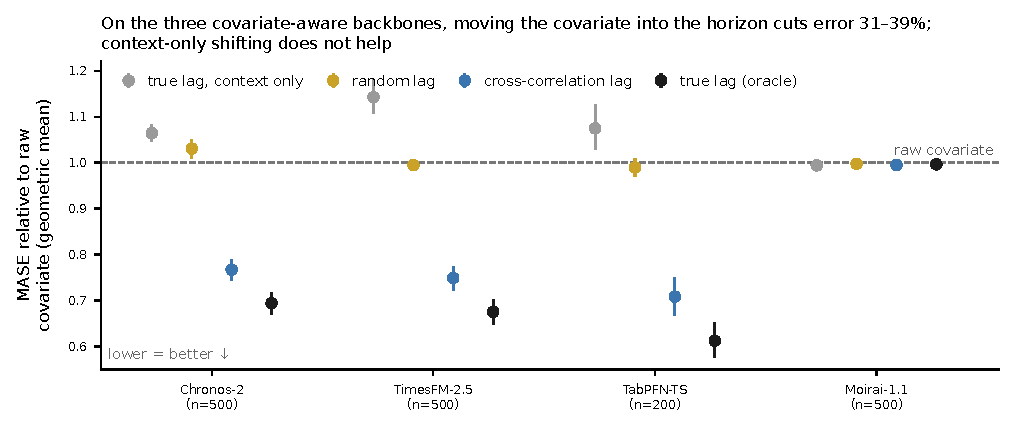
\includegraphics[width=\linewidth]{figs/fig1_gate.pdf}
\caption{Headroom gate (dev split, ten cells, $C=512$, $H=24$). Points are geometric means of per-series MASE ratios relative to the raw past covariate, with 95\% bootstrap intervals over series; $n$ is the number of series (TabPFN-TS: 20 per cell). ``True lag, context only'' shifts the covariate in the context but leaves the horizon missing.}
\label{fig:gate}
\end{figure}

\begin{table}[t]\centering\small
\caption{Pre-registered headroom gate (dev split; GM-MASE). G1: GM[oracle/ref] $\le 0.95$ with Wilcoxon $p<0.01$, ref = better of no covariate and raw covariate. G2: GM[random lag/oracle] $\ge 1.05$. ``Context only'': true-lag shift in the context, horizon left missing.}
\label{tab:gate}
\resizebox{\linewidth}{!}{\begin{tabular}{lrrrrrrrrrrc}
\toprule
Backbone & $n$ & no cov. & raw & context only & random lag & CCF & oracle & G1 ratio & $p$ & G2 ratio & pass \\
\midrule
Chronos-2 & 500 & 0.663 & 0.617 & 0.656 & 0.636 & 0.473 & 0.428 & 0.694 & $<10^{-10}$ & 1.485 & yes \\
TimesFM-2.5 & 500 & 0.659 & 0.663 & 0.757 & 0.659 & 0.496 & 0.447 & 0.679 & $<10^{-10}$ & 1.473 & yes \\
TabPFN-TS & 200 & 0.697 & 0.694 & 0.746 & 0.687 & 0.492 & 0.425 & 0.613 & $<10^{-10}$ & 1.615 & yes \\
Moirai-1.1 & 500 & 0.679 & 0.690 & 0.685 & 0.688 & 0.686 & 0.687 & 1.012 & 0.069 & 1.001 & no \\
\bottomrule
\end{tabular}}
\end{table}

\subsection{Learned alignment on held-out synthetic tasks}
\label{sec:synth}

Table~\ref{tab:synth} and Figure~\ref{fig:synth} compare \lta{} with classical shifting on the 1,300 test series (Chronos-2 backbone). Averaged over all families, \lta{} lowered GM-MASE relative to the cross-correlation shift by 3.7--4.0\% across three seeds ($p<10^{-25}$ for seed 0). The gains were concentrated where the gate located the gap. For time-varying leads the ratio to cross-correlation was 0.907--0.923, and for distributed responses 0.903--0.917 (pulse), where \lta{} was even 8\% more accurate than the point-lag oracle (seed 0, ratio 0.920). The oracle shifts by a single lag, whereas the soft splat can spread a pulse over its response kernel. For nonlinear responses the ratio was 0.972--0.977. For linear and periodic fixed leads and for the uninformative covariate it was 0.995--1.001, so \lta{} did no harm where classical alignment is already optimal. For time-varying leads \lta{} recovered only about a fifth of the remaining gap to the oracle (oracle/cross-correlation 0.663), so state-dependent lead estimation from 512 context steps is far from solved.

The ablations (Figure~\ref{fig:synth}, Table~\ref{tab:ablation}) attribute the gains:
\begin{itemize}
\item Removing the state-dependent offset eliminated the gain on time-varying leads (0.989) but slightly improved pulses (0.882), so the offset head is what tracks varying leads. Its validation-selected checkpoint was at step 250, i.e.\ this variant barely moved from its cross-correlation initialisation, and its comparison should be read with that in mind (selected steps of the other ablations: 1,000 without CCF initialisation, 3,000 without auxiliary losses).
\item Removing the cross-correlation initialisation also eliminated the time-varying gain (0.990).
\item Removing the auxiliary losses reduced it (0.972) and degraded transfer to rivers (below).
\end{itemize}

\paragraph{Transfer on synthetic tasks} The same three aligners, trained through Chronos-2 only, were applied without retraining to TimesFM-2.5 and TabPFN-TS on the same test series (Table~\ref{tab:synth_transfer}; P5). On both backbones \lta{} beat the cross-correlation shift for every seed: by 3.1--3.6\% with TimesFM-2.5 (Wilcoxon $p<10^{-14}$) and by 6.7\% with TabPFN-TS ($p<10^{-20}$). The gains fell where they fell for Chronos-2. With TimesFM-2.5 they were concentrated on time-varying leads (0.870--0.887). With TabPFN-TS they appeared for time-varying leads (0.882), distributed responses (0.870) and nonlinear responses (0.891). On fixed linear and periodic leads and on the uninformative covariate, \lta{} matched the cross-correlation shift on all three backbones (0.989--1.002). Learned alignment is therefore not specific to the backbone it was trained through: on synthetic data its advantage carries over to two backbones with different covariate mechanisms.

\begin{table}[t]\centering\small
\caption{Held-out synthetic test set on three frozen backbones. The aligned covariates come from the same three synthetic-only \lta{} seeds, trained through Chronos-2 only. Columns 3--4: GM-MASE ratios of the plain cross-correlation shift and of the oracle shift relative to the raw covariate (seed-independent). Remaining columns: GM of per-series MASE ratios \lta{}/cross-correlation shift, range over seeds (one seed for TabPFN-TS), overall and by family; $p$: largest Wilcoxon $p$ over seeds. TabPFN-TS uses 50 of the 100 series per cell.}
\label{tab:synth_transfer}
\resizebox{\linewidth}{!}{\begin{tabular}{lrrrllllllll}
\toprule
 & & \multicolumn{2}{c}{vs raw} & \multicolumn{8}{c}{\lta{} / cross-correlation shift} \\ \cmidrule(lr){3-4}\cmidrule(lr){5-12}
Backbone & $n$ & CCF & oracle & all & $p$ & fixed, linear & fixed, periodic & fixed, nonlinear & distributed & time-varying & uninformative \\
\midrule
Chronos-2 & 1300 & 0.815 & 0.735 & 0.960--0.963 & $<10^{-27}$ & 1.000--1.001 & 0.998 & 0.972--0.977 & 0.903--0.917 & 0.907--0.923 & 0.995--1.000 \\
TimesFM-2.5 & 1300 & 0.790 & 0.707 & 0.964--0.969 & $<10^{-14}$ & 1.001--1.002 & 0.997 & 0.991--0.992 & 0.981--0.984 & 0.870--0.887 & 0.989--0.997 \\
TabPFN-TS & 650 & 0.752 & 0.643 & 0.933 & $<10^{-20}$ & 1.001 & 0.989 & 0.891 & 0.870 & 0.882 & 1.002 \\
\bottomrule
\end{tabular}}
\end{table}

\begin{figure}[t]
\centering
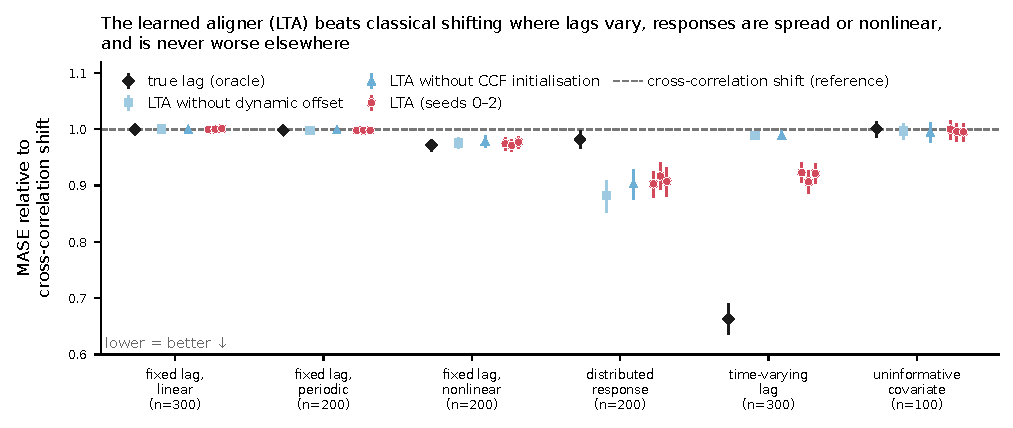
\includegraphics[width=\linewidth]{figs/fig2_synth.pdf}
\caption{Held-out synthetic test set (Chronos-2). Geometric mean of per-series MASE ratios relative to per-window cross-correlation shifting, with 95\% bootstrap intervals over series. Three \lta{} seeds are shown side by side. ``Distributed response'': gamma-kernel pulse response; ``time-varying lag'': lead shortens with the system state.}
\label{fig:synth}
\end{figure}

\begin{table}[t]\centering\small
\caption{Held-out synthetic test set (Chronos-2). Left: GM-MASE. Right: GM of per-series MASE ratios relative to CCF shifting; LTA range over three seeds; $p$: Wilcoxon, LTA seed 0 vs CCF.}
\label{tab:synth}
\resizebox{\linewidth}{!}{\begin{tabular}{lrrrrrrr|rrr}
\toprule
 & & \multicolumn{6}{c|}{GM-MASE} & \multicolumn{3}{c}{ratio to CCF} \\
Family & $n$ & raw & CCF & top-3 & GCC-PHAT & oracle & LTA & oracle & LTA (seeds) & $p$ \\
\midrule
fixed lag, linear & 300 & 0.544 & 0.420 & 0.428 & 0.420 & 0.420 & 0.420 & 1.000 & 1.000--1.001 & 0.942 \\
fixed lag, periodic & 200 & 0.666 & 0.460 & 0.479 & 0.459 & 0.459 & 0.459 & 0.998 & 0.998--0.998 & 0.191 \\
fixed lag, nonlinear & 200 & 0.648 & 0.488 & 0.520 & 0.492 & 0.475 & 0.476 & 0.972 & 0.972--0.977 & $5.0\times10^{-5}$ \\
distributed response & 200 & 0.529 & 0.479 & 0.464 & 0.478 & 0.470 & 0.432 & 0.982 & 0.903--0.917 & $<10^{-10}$ \\
time-varying lag & 300 & 0.674 & 0.590 & 0.589 & 0.615 & 0.391 & 0.544 & 0.663 & 0.907--0.923 & $<10^{-10}$ \\
uninformative & 100 & 0.719 & 0.733 & 0.740 & 0.730 & 0.734 & 0.734 & 1.001 & 0.995--1.000 & 0.514 \\
all & 1300 & 0.616 & 0.502 & 0.510 & 0.507 & 0.453 & 0.483 & 0.903 & 0.960--0.963 & $<10^{-10}$ \\
\bottomrule
\end{tabular}}
\end{table}

\begin{table}[t]\centering\small
\caption{Ablations (Chronos-2). Synthetic: GM ratio to CCF shifting on the test set. RiverLead: pooled ratio to the best classical arm (top3) with block-bootstrap 95\% interval and pairs improved (of 9).}
\label{tab:ablation}
\resizebox{\linewidth}{!}{\begin{tabular}{lrrrrrlr}
\toprule
 & \multicolumn{4}{c}{synthetic, ratio to CCF} & \multicolumn{3}{c}{RiverLead, ratio to best classical} \\
Variant & time-varying & distributed & nonlinear & all & ratio & 95\% CI & pairs \\
\midrule
full model (seed 0) & 0.923 & 0.903 & 0.974 & 0.962 & 0.984 & [0.977, 0.991] & 8/9 \\
no state-dependent offset & 0.989 & 0.882 & 0.976 & 0.974 & 0.992 & [0.985, 0.999] & 6/9 \\
no CCF initialisation & 0.990 & 0.904 & 0.979 & 0.979 & 0.990 & [0.984, 0.997] & 7/9 \\
no auxiliary losses & 0.972 & 0.850 & 0.972 & 0.965 & 1.026 & [1.017, 1.034] & 2/9 \\
\bottomrule
\end{tabular}}
\end{table}

\subsection{RiverLead: alignment helps, learned alignment adds little}
\label{sec:river}

Table~\ref{tab:river} reports the pre-registered RiverLead evaluation with Chronos-2. The raw past covariate already helped (5.4\% lower GM-MASE than no covariate). Aligning it helped further: the best classical arm selected on validation, top-3 cross-correlation peaks, lowered GM-MASE by a further 8.2\% (ratio 0.918, 95\% CI [0.906, 0.929], 8/9 pairs). Hypothesis H1 is therefore supported for Chronos-2. Prewhitened cross-correlation (0.915) and the flow-binned training lag (0.918, 9/9 pairs) were statistically indistinguishable from top-3 peaks. A single global lag per pair (0.932) and per-window raw cross-correlation (0.933) were somewhat worse, and GCC-PHAT, whose phase transform whitens away the low-frequency hydrograph, captured little (0.987). The random-lag control did not help (1.005, CI [0.995, 1.015]), so the gains require the lag to be right and do not come from adding a horizon-filled channel. Figure~\ref{fig:real} shows the per-pair results. Gains were larger on event windows, those with a rapid upstream change, where the best classical arm reached 0.906 and \lta{} seed 0 reached 0.879 relative to the raw covariate. Figure~\ref{fig:arch}b shows a Delaware flood in the test period. The raw covariate forecast a flat recession, the cross-correlation shift captured part of the rise, and the \lta{}-aligned covariate captured most of it.

Hypothesis H2, that \lta{} beats the best classical arm, was supported for the pre-registered seed 0 (ratio 0.984, CI [0.977, 0.991], 8/9 pairs) but not for seeds 1 and 2 (0.998 each, CIs including 1, 5/9 and 4/9 pairs). We therefore do not claim that learned alignment improves on classical alignment for rivers; the effect ranges from 0.2\% to 1.6\% depending on the seed. Fine-tuning the aligner on river data never improved validation error over the synthetic-only aligner, so early stopping returned the zero-shot weights in every run (D4). The leave-one-pair-out aligners are therefore the synthetic-only aligner, with test errors identical to within $4\times10^{-5}$ MASE. H3 is formally met (0.984, CI [0.977, 0.991]), but only trivially: an aligner that has seen no river data transfers to every held-out pair. This adds no evidence beyond H2. The ablations (Table~\ref{tab:ablation}) show the same picture: on rivers no variant was clearly better than the full model, and removing the auxiliary oracle losses made \lta{} 2.6\% \emph{worse} than classical alignment, although that variant did well on synthetic pulses. This suggests that supervision towards the correct lag during synthetic training is what lets the aligner transfer to real data, although it rests on a single run of the ablated variant.

Fine-tuning Chronos-2 itself on six years of training data with the raw covariate was more accurate than any frozen arm (full: 0.808 relative to raw; LoRA: 0.797). Relative to the best classical alignment this is a further 12--13\% reduction, in all nine pairs. When a long in-domain history exists and the model may be modified, fine-tuning remains preferable. Frozen alignment is the option when weights cannot be changed, when one model serves many sites, or when the history is short. We did not evaluate fine-tuning combined with alignment, which would be the natural next step.

\begin{table}[t]\centering\small
\caption{RiverLead test split (Chronos-2 backbone; 9 pairs, \num{9046} windows). GM-MASE pooled over pairs; ratios with 7-day block-bootstrap 95\% intervals and number of pairs improved. The best classical arm on validation was top3. Fine-tuned rows modify the backbone and use the training split.}
\label{tab:river}
\resizebox{\linewidth}{!}{\begin{tabular}{lrrlrrlr}
\toprule
Arm & GM-MASE & \multicolumn{3}{c}{ratio to raw} & \multicolumn{3}{c}{ratio to best classical} \\
\midrule
no covariate & 0.286 & 1.057 & [1.050, 1.063] & 0/9 & 1.151 & [1.136, 1.167] & 0/9 \\
raw past covariate & 0.271 & -- & -- & -- & 1.090 & [1.077, 1.104] & 1/9 \\
random lag (control) & 0.272 & 1.005 & [0.995, 1.015] & 3/9 & 1.095 & [1.082, 1.108] & 0/9 \\
GCC-PHAT & 0.267 & 0.987 & [0.984, 0.991] & 7/9 & 1.076 & [1.063, 1.089] & 1/9 \\
CCF & 0.253 & 0.933 & [0.924, 0.943] & 8/9 & 1.017 & [1.011, 1.023] & 2/9 \\
global train lag & 0.252 & 0.932 & [0.924, 0.941] & 8/9 & 1.016 & [1.007, 1.024] & 3/9 \\
CCF, prewhitened & 0.248 & 0.915 & [0.905, 0.925] & 8/9 & 0.997 & [0.990, 1.003] & 5/9 \\
top-3 CCF peaks & 0.248 & 0.918 & [0.906, 0.929] & 8/9 & -- & -- & -- \\
flow-binned train lag & 0.249 & 0.918 & [0.908, 0.928] & 9/9 & 1.001 & [0.993, 1.007] & 5/9 \\
LTA, seed 0 & 0.245 & 0.903 & [0.893, 0.913] & 8/9 & 0.984 & [0.977, 0.991] & 8/9 \\
LTA, seed 1 & 0.248 & 0.916 & [0.906, 0.926] & 8/9 & 0.998 & [0.992, 1.005] & 5/9 \\
LTA, seed 2 & 0.248 & 0.916 & [0.906, 0.926] & 8/9 & 0.998 & [0.990, 1.006] & 4/9 \\
fine-tuned Chronos-2 (full), raw & 0.219 & 0.808 & [0.796, 0.821] & 9/9 & 0.880 & [0.869, 0.891] & 9/9 \\
fine-tuned Chronos-2 (LoRA), raw & 0.216 & 0.797 & [0.784, 0.810] & 9/9 & 0.868 & [0.858, 0.879] & 9/9 \\
\bottomrule
\end{tabular}}
\end{table}

\begin{figure}[t]
\centering
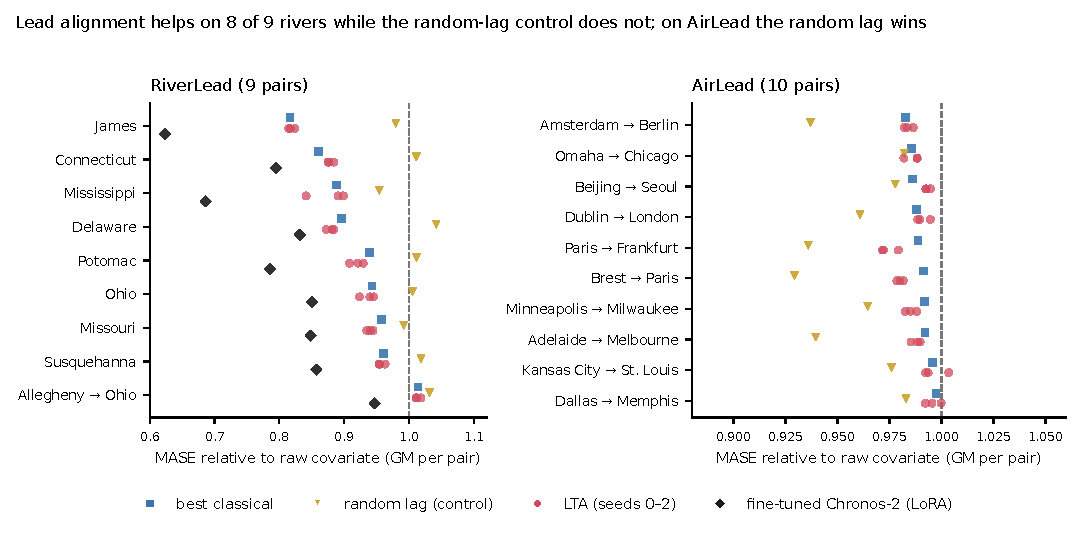
\includegraphics[width=\linewidth]{figs/fig3_real.pdf}
\caption{Per-pair test results with Chronos-2: geometric mean MASE ratio relative to the raw past covariate for each gauge or station pair (left: RiverLead; right: AirLead, note the narrower $x$-range). Best classical arm selected on validation (RiverLead: top-3 CCF peaks; AirLead: prewhitened CCF). Fine-tuning modifies the backbone and was run on RiverLead only.}
\label{fig:real}
\end{figure}

\subsection{AirLead: a cautionary second domain}
\label{sec:air}

Table~\ref{tab:air} reports the pre-registered AirLead evaluation. For Chronos-2 the raw upwind covariate lowered GM-MASE by 4.4\% relative to no covariate, and the best classical arm on validation, prewhitened cross-correlation, lowered it by a further 1.0\% (ratio 0.990, CI [0.987, 0.993], 10/10 pairs), so W1 is formally supported. \lta{} seed 0 was 0.4\% better than this arm (0.996, CI [0.993, 1.000], 7/10 pairs), which formally meets W2, but seed 1 (0.999, CI [0.996, 1.003]) did not, so W2-robust is not supported and we claim no learned-alignment benefit on AirLead. With TimesFM-2.5, the pre-registered classical arm (prewhitened cross-correlation, selected on Chronos-2 validation) lowered GM-MASE by 7.0\% relative to the raw covariate (0.930, CI [0.921, 0.938], 10/10 pairs), so W1 holds for both backbones. All three \lta{} seeds beat this arm (ratios 0.926, 0.922 and 0.933; CIs exclude 1; 10, 10 and 8 of 10 pairs), so W3 is supported. However, top-3 cross-correlation peaks, which were run on TimesFM-2.5 but were not the pre-registered comparator, were better still: \lta{} was 1.8--3.1\% worse than top-3 for every seed (seed 0: 1.023, CI [1.015, 1.032], 2/10 pairs). With TimesFM-2.5, then, alignment of any kind helps markedly on AirLead (14--16\% relative to raw). The learned aligner beats a single classical lag but not a three-lag bank. The post-hoc controls (D12, D13) qualify this. Unlike Chronos-2, TimesFM-2.5 did not benefit from a random lag (1.011 relative to raw, CI [1.005, 1.016], 2/10 pairs). Every aligned arm beat the random lag in all ten pairs: prewhitened CCF by 8.0\%, top-3 by 16.7\% and \lta{} by 14.1--15.2\% across seeds. With TimesFM-2.5, the AirLead gains are therefore lead-specific. But as on rivers, the raw upwind covariate was harmful through XReg (28.8\% worse than no covariate, CI [1.265, 1.310], 0/10 pairs), and even the best aligned arm remained 8.4\% worse than no covariate (top-3: 1.084, CI [1.063, 1.103]).

The pre-registered random-lag control changes the interpretation of these small gains. On AirLead (Figure~\ref{fig:real}, right) a random lag in $[24,168]$\,h was more accurate than every aligned arm (0.958 relative to raw, 10/10 pairs; 0.972 relative to \lta{} seed 0), whereas on RiverLead it had no effect. A post-hoc check on the validation split (Table~\ref{tab:air_explo}) showed that fixed lags of 48--168\,h and even an i.i.d.\ noise channel known over the horizon also lowered Chronos-2 error, by 1--4\%. On AirLead, therefore, Chronos-2 benefits from the \emph{presence} of a horizon-filled known covariate, independently of its content. The 1\% gain from correct alignment cannot be separated from this generic effect. We see two plausible reasons. Pressure fields are spatially coherent, so much of the upwind--downwind covariation is simultaneous and the lead carries little additional information over a 24-hour horizon. In addition, adding a known covariate appears to change how Chronos-2 extrapolates a smooth target, regardless of what the covariate contains. We did not test either explanation further. The practical lesson is that covariate gains reported for TSFMs should be benchmarked against random-lag or noise controls. Without the control, AirLead would have appeared to confirm alignment, and with it AirLead neither confirms nor refutes it.

\begin{table}[t]\centering\small
\caption{AirLead test split (10 pairs, \num{10960} windows). Pooled GM-MASE ratios with 7-day block-bootstrap 95\% intervals and pairs improved (of 10). Best classical arm on validation (Chronos-2): ccf\_pw. The random-lag row is the pre-registered specificity control.}
\label{tab:air}
\resizebox{\linewidth}{!}{\begin{tabular}{lrrlrrlr}
\toprule
 & \multicolumn{4}{c}{Chronos-2} & \multicolumn{3}{c}{TimesFM-2.5 (XReg)} \\
Arm & GM-MASE & ratio to raw & 95\% CI & pairs & GM-MASE & ratio to raw & pairs \\
\midrule
no covariate & 0.365 & 1.046 & [1.041, 1.050] & 0/10 & 0.367 & 0.777 & 10/10 \\
raw past covariate & 0.349 & -- & -- & -- & 0.473 & -- & -- \\
random lag (control) & 0.334 & 0.958 & [0.952, 0.965] & 10/10 & 0.478 & 1.011 & 2/10 \\
GCC-PHAT & 0.346 & 0.993 & [0.991, 0.995] & 9/10 & -- & -- & -- \\
CCF & 0.345 & 0.990 & [0.985, 0.995] & 10/10 & -- & -- & -- \\
global train lag & 0.346 & 0.991 & [0.989, 0.994] & 10/10 & -- & -- & -- \\
CCF, prewhitened & 0.345 & 0.990 & [0.987, 0.993] & 10/10 & 0.439 & 0.930 & 10/10 \\
top-3 CCF peaks & 0.348 & 0.999 & [0.992, 1.005] & 6/10 & 0.398 & 0.842 & 10/10 \\
level-binned train lag & 0.346 & 0.992 & [0.989, 0.995] & 9/10 & 0.443 & 0.938 & 8/10 \\
LTA, seed 0 & 0.344 & 0.986 & [0.981, 0.991] & 10/10 & 0.407 & 0.861 & 10/10 \\
LTA, seed 1 & 0.345 & 0.989 & [0.984, 0.994] & 9/10 & 0.405 & 0.857 & 10/10 \\
LTA, seed 2 & 0.344 & 0.987 & [0.982, 0.992] & 10/10 & 0.410 & 0.868 & 10/10 \\
\bottomrule
\end{tabular}}
\end{table}

\subsection{Transfer of the aligned covariate to other backbones}
\label{sec:transfer}

The aligned covariates produced by the synthetic-only \lta{} (seed 0, trained through Chronos-2) were passed unchanged to the other backbones on the RiverLead test split (Table~\ref{tab:transfer}). For reference, with Chronos-2 the raw covariate lowered GM-MASE by 5.4\% relative to no covariate, and \lta{} plus the raw covariate by 14.5\% (0.855, CI [0.844, 0.866], 9/9 pairs).

TimesFM-2.5 behaved differently. Through XReg, the raw past river covariate made forecasts 32.9\% \emph{worse} than no covariate (1.329, CI [1.294, 1.367], 0/9 pairs). Alignment removed most of this harm, and the reduction was lead-specific:
\begin{itemize}
\item A random lag (post hoc, D13) gave no improvement over raw (1.004, CI [0.993, 1.017]).
\item The best classical arm lowered GM-MASE by 18.7\% relative to raw (flow-binned lag: 0.813, CI [0.797, 0.831], 8/9 pairs) but remained 8.1\% worse than no covariate.
\item \lta{} lowered it by 24.5\% (0.755, CI [0.739, 0.772], 8/9 pairs) and reached parity with no covariate (1.004, CI [0.980, 1.031], 4/9 pairs).
\end{itemize}
Against classical alignment, the synthetic-only aligner was better than the arm selected on Chronos-2 validation (top-3 peaks: 0.891, CI [0.878, 0.904], 8/9 pairs). It was also better than the classical arm that was best on TimesFM's own \emph{test} data, a choice that favours the baseline (flow-binned lag: 0.929, CI [0.917, 0.941], 7/9 pairs; the exceptions were Delaware, 1.032, and Allegheny--Ohio, 1.022). The TimesFM-2.5 run covered only the test split, so the pre-registered validation-based selection could not be made for this backbone. In short, with TimesFM-2.5 learned alignment beats classical and random alignment by a clear margin, but on these rivers it only neutralises the damage that the XReg interface does with a past-only covariate; it does not make the covariate useful. A plausible reason is that XReg fits a same-time linear regression on the context and extrapolates it over the horizon, which is fragile for heavy-tailed, non-stationary discharge; we did not test this. Only one aligner seed was transferred, so seed variation on TimesFM-2.5 is not assessed.

\begin{table}[t]\centering\small
\caption{Transfer on the RiverLead test split. The same aligned covariates (synthetic-only \lta{}, seed 0, trained through Chronos-2) are fed to every backbone. Each cell: pooled GM-MASE ratio (pairs improved of 9) with block-bootstrap 95\% interval below. ``Best classical'' is chosen on each backbone's \emph{test} split among prewhitened CCF, top-3 peaks and the flow-binned lag, which favours the baseline. TabPFN-TS uses every 4th window (D5). The TimesFM-2.5 no-covariate arm is the corrected one (D12) and its random-lag control is post hoc (D13); random lag was not run for TabPFN-TS and Moirai-1.1.}
\label{tab:transfer}
\setlength{\tabcolsep}{4pt}\begin{tabular}{lcccc}
\toprule
Ratio & Chronos-2 & TimesFM-2.5 & TabPFN-TS & Moirai-1.1 \\
 & $n=9046$ & $n=9046$ & $n=2262$ & $n=9046$ \\
\midrule
raw / no cov. & 0.946 (9/9) & 1.329 (0/9) & 1.245 (0/9) & 1.134 (0/9) \\
 & {\footnotesize [0.941, 0.952]} & {\footnotesize [1.294, 1.367]} & {\footnotesize [1.195, 1.297]} & {\footnotesize [1.115, 1.156]} \\[2pt]
random lag / raw & 1.005 (3/9) & 1.004 (4/9) & -- & -- \\
 & {\footnotesize [0.995, 1.015]} & {\footnotesize [0.993, 1.017]} & {\footnotesize } & {\footnotesize } \\[2pt]
best class. / raw & 0.915 (8/9) & 0.813 (8/9) & 1.008 (4/9) & 1.017 (0/9) \\
 & {\footnotesize [0.905, 0.925]} & {\footnotesize [0.797, 0.831]} & {\footnotesize [0.975, 1.042]} & {\footnotesize [1.011, 1.022]} \\[2pt]
\lta{} / raw & 0.903 (8/9) & 0.755 (8/9) & 1.022 (4/9) & 1.019 (0/9) \\
 & {\footnotesize [0.893, 0.913]} & {\footnotesize [0.739, 0.772]} & {\footnotesize [0.989, 1.057]} & {\footnotesize [1.012, 1.025]} \\[2pt]
\lta{} / best class. & 0.987 (8/9) & 0.929 (7/9) & 1.015 (3/9) & 1.002 (4/9) \\
 & {\footnotesize [0.981, 0.994]} & {\footnotesize [0.917, 0.941]} & {\footnotesize [0.998, 1.032]} & {\footnotesize [0.999, 1.004]} \\[2pt]
\lta{} / top-3 & 0.984 (8/9) & 0.891 (8/9) & 1.003 (3/9) & 0.990 (8/9) \\
 & {\footnotesize [0.977, 0.991]} & {\footnotesize [0.878, 0.904]} & {\footnotesize [0.981, 1.023]} & {\footnotesize [0.986, 0.993]} \\[2pt]
\lta{} / no cov. & 0.855 (9/9) & 1.004 (4/9) & 1.273 (2/9) & 1.156 (0/9) \\
 & {\footnotesize [0.844, 0.866]} & {\footnotesize [0.980, 1.031]} & {\footnotesize [1.207, 1.345]} & {\footnotesize [1.135, 1.176]} \\[2pt]
\midrule
best classical arm & CCF-pw & binned & binned & binned \\
\bottomrule
\end{tabular}
\end{table}

TabPFN-TS and Moirai-1.1 behaved differently (Table~\ref{tab:transfer}). For both, adding the raw past river covariate made forecasts worse than using no covariate at all: by 24.5\% for TabPFN-TS (ratio 1.245, CI [1.195, 1.297]) and by 13.4\% for Moirai-1.1 (1.134, CI [1.115, 1.156]), in all nine pairs. Neither classical nor learned alignment recovered this loss. For TabPFN-TS, every aligned arm was within 2\% of the raw covariate, with intervals that include 1. For Moirai-1.1, the aligned arms were 1.7--1.9\% worse than raw; top-3 peaks were the exception, slightly worse than \lta{} (\lta{}/top-3 0.990). For Moirai this agrees with the gate, where the backbone ignored even an oracle-shifted covariate. For TabPFN-TS it does not: the gate showed 39\% headroom on synthetic data. Every aligned arm in our design also carries the raw past covariate, which damages TabPFN-TS on rivers, so the benefit of the aligned channel may be masked by that harm. We did not test an arm without the raw channel. We therefore do not claim that alignment helps TabPFN-TS or Moirai-1.1 on real data. Across the four backbones, only with Chronos-2 did a covariate arm beat the no-covariate forecast on real rivers. With TimesFM-2.5, learned alignment restored parity; with TabPFN-TS and Moirai-1.1 the past covariate remained harmful.

\subsection{EnergyLead: a domain without a usable lead}
\label{sec:energy}

EnergyLead was added in the revision protocol as a third physical domain (P5). Its premise, that wind generation in a downwind area lags generation in the upwind neighbour by an advection time, was not borne out (Table~\ref{tab:energy}). The training-split global lag was 0\,h for seven pairs, 1--2\,h for two and 8\,h for Ireland$\to$Great Britain. An aligned channel with lag 0 contains no horizon values, so on this benchmark most ``aligned'' arms are a second copy of the past covariate. Area-aggregated generation integrates many sites, and over areas of a few hundred kilometres the shared weather signal is largely simultaneous at hourly resolution.

The hypothesis tests reflect this. For Chronos-2, the raw upwind covariate lowered GM-MASE by 1.8\% relative to no covariate (0.982, CI [0.979, 0.986], 9/10 pairs). The classical arm selected on validation (the global lag) improved on raw by only 0.4\% (0.996, CI [0.993, 0.999], 9/10), so E1 is formally met, although the gain cannot be attributed to alignment. All three \lta{} seeds were 1.8--2.0\% worse than this arm (1--2 of 10 pairs better), so E2 is not supported. \lta{} was also 1.4\% worse than the raw covariate (seed 0: 1.014, CI [1.007, 1.021]), which is consistent with its imposing leads that the data do not contain; we did not inspect its estimated leads. The random lag was worse still (1.038 relative to raw, 0/10 pairs), so E3 holds only in the trivial sense that every aligned arm beat a harmful control. With TimesFM-2.5 every arm except the random lag (1.016) was within 1\% of the raw covariate (0.996--1.010), so E1 fails for this backbone, and no arm beat the no-covariate forecast (raw relative to no covariate: 1.012, CI [1.000, 1.025]).

EnergyLead therefore marks a boundary of the approach. When the lead is shorter than a few time steps, input alignment has nothing to move into the horizon. The learned aligner then does mild harm, so it is not a substitute for checking whether a lead exists. In this situation, a trained adapter that re-weights the covariate is the more useful frozen-backbone tool (Section~\ref{sec:cross}).

\begin{table}[t]\centering\small
\caption{EnergyLead test split (10 pairs, \num{6313} windows; P5). Pooled GM-MASE ratios with 7-day block-bootstrap 95\% intervals and pairs improved (of 10). Best classical arm on validation (Chronos-2): global. The fitted global train lags are 0--2\,h for nine of ten pairs (Ireland$\to$GB: 8\,h).}
\label{tab:energy}
\resizebox{\linewidth}{!}{\begin{tabular}{lrrlrrlr}
\toprule
 & \multicolumn{4}{c}{Chronos-2} & \multicolumn{3}{c}{TimesFM-2.5 (XReg)} \\
Arm & GM-MASE & ratio to raw & 95\% CI & pairs & GM-MASE & ratio to raw & pairs \\
\midrule
no covariate & 0.538 & 1.018 & [1.014, 1.022] & 1/10 & 0.546 & 0.988 & 6/10 \\
raw past covariate & 0.529 & -- & -- & -- & 0.553 & -- & -- \\
random lag (control) & 0.549 & 1.038 & [1.028, 1.048] & 0/10 & 0.562 & 1.016 & 1/10 \\
GCC-PHAT & 0.530 & 1.003 & [0.999, 1.007] & 4/10 & 0.555 & 1.004 & 5/10 \\
CCF & 0.532 & 1.006 & [1.000, 1.012] & 3/10 & 0.551 & 0.996 & 6/10 \\
global train lag & 0.527 & 0.996 & [0.993, 0.999] & 9/10 & 0.553 & 1.000 & 7/10 \\
CCF, prewhitened & 0.534 & 1.010 & [1.004, 1.015] & 4/10 & 0.554 & 1.001 & 7/10 \\
top-3 CCF peaks & 0.541 & 1.022 & [1.012, 1.031] & 2/10 & 0.552 & 0.998 & 5/10 \\
level-binned train lag & 0.531 & 1.003 & [0.999, 1.008] & 6/10 & 0.555 & 1.004 & 3/10 \\
LTA, seed 0 & 0.536 & 1.014 & [1.007, 1.021] & 3/10 & 0.557 & 1.007 & 4/10 \\
LTA, seed 1 & 0.537 & 1.016 & [1.008, 1.024] & 3/10 & 0.554 & 1.003 & 4/10 \\
LTA, seed 2 & 0.537 & 1.015 & [1.007, 1.022] & 3/10 & 0.558 & 1.010 & 2/10 \\
\bottomrule
\end{tabular}}
\end{table}

\subsection{TrafficLead: a multi-step but weak lead}
\label{sec:traffic}

TrafficLead was added to test a second domain with a physical lead of several steps (P6). The results are again negative for alignment (Table~\ref{tab:traffic}). With Chronos-2 the raw downstream speed lowered GM-MASE by 2.1\% relative to no covariate (0.979, CI [0.974, 0.985], 9/10 pairs). The classical arm selected on validation, the level-binned lag, was 1.1\% \emph{worse} than the raw covariate (1.011, CI [1.006, 1.015], 3/10 pairs), so T1 fails, and all three \lta{} seeds were 0.7--1.1\% worse than that arm, so T2 fails. The random lag was worse still (1.015), and even the aligned arm that was best on test, the global lag, did not beat it clearly (0.994, CI [0.988, 1.002]), so T3 fails as well. The six pairs without imputed sensors give the same picture (raw/no covariate 0.978; level-binned/raw 1.015, CI [1.009, 1.021], 1/6 pairs; \lta{}/raw 1.018), as does the subset of five pairs with training lags of 3--29 steps (level-binned/raw 1.020, \lta{}/raw 1.019). With TimesFM-2.5 the raw downstream speed was harmful, as it was on rivers (1.283 relative to no covariate, CI [1.269, 1.297], 0/10 pairs; filtered pairs 1.348), and every aligned arm was worse still (1.115--1.163 relative to raw), as was the random lag (1.123). The three \lta{} seeds beat the level-binned lag by 0.7--1.6\% (CIs exclude 1, 7/10 pairs), so T2 is formally met for TimesFM-2.5, but only relative to a classical arm that is itself harmful: \lta{} remained 12.0--13.0\% worse than the raw covariate and 43.7--45.0\% worse than no covariate. T1 fails, and T3 fails on the pre-registered pairs (best aligned arm on test against the random lag: 0.993, CI [0.984, 1.001]).

The training-split diagnostic in Table~\ref{tab:leaddiag} offers a plausible reading. The lead in TrafficLead is long but weak: the mean cross-correlation peak at the training lag is 0.08--0.11, against 0.15--0.61 for RiverLead. We conjecture that five-minute speeds are dominated by the target's own daily pattern and by local noise, so that the shifted downstream speed adds little that the target's history does not already contain; we did not test this directly. Only RiverLead combines a multi-step lead with a non-trivial correlation at that lag. AirLead has a strong but essentially simultaneous relation (median training lag 0, correlation 0.51) and EnergyLead a moderate simultaneous one (0.21). This diagnostic is post hoc (D24) and rests on four domains, so we offer it as a heuristic, not a validated rule.

\begin{table}[t]\centering\small
\caption{TrafficLead test split (PEMS-BAY, 5-min speeds; P6). Pooled GM-MASE ratios to the raw covariate with 7-day block-bootstrap 95\% intervals and pairs improved. `All': the ten pre-registered pairs (\num{7320} windows); `filtered': the six pairs without imputed sensors (D25). Best classical arm on Chronos-2 validation: level-binned train lag. Train global lags: 3--29 steps for five pairs and 103--112 steps for the other five (D22).}
\label{tab:traffic}
\resizebox{\linewidth}{!}{\begin{tabular}{lrrlrrrrr}
\toprule
 & \multicolumn{6}{c}{Chronos-2} & \multicolumn{2}{c}{TimesFM-2.5 (XReg)} \\ \cmidrule(lr){2-7}\cmidrule(lr){8-9}
Arm & GM-MASE & ratio (all) & 95\% CI & pairs & ratio (filtered) & pairs & ratio (all) & ratio (filtered) \\
\midrule
no covariate & 0.299 & 1.021 & [1.016, 1.027] & 1/10 & 1.022 & 0/6 & 0.779 & 0.742 \\
raw past covariate & 0.293 & -- & -- & -- & -- & -- & -- & -- \\
random lag (control) & 0.297 & 1.015 & [1.009, 1.022] & 0/10 & 1.017 & 0/6 & 1.123 & 1.078 \\
GCC-PHAT & 0.299 & 1.020 & [1.014, 1.026] & 0/10 & 1.018 & 0/6 & 1.133 & 1.069 \\
CCF & 0.296 & 1.011 & [1.008, 1.015] & 2/10 & 1.011 & 2/6 & 1.145 & 1.080 \\
global train lag & 0.296 & 1.010 & [1.005, 1.014] & 4/10 & 1.015 & 2/6 & 1.141 & 1.081 \\
CCF, prewhitened & 0.299 & 1.019 & [1.012, 1.027] & 1/10 & 1.023 & 0/6 & 1.115 & 1.071 \\
top-3 CCF peaks & 0.300 & 1.025 & [1.021, 1.030] & 1/10 & 1.024 & 1/6 & 1.163 & 1.092 \\
level-binned train lag & 0.296 & 1.011 & [1.006, 1.015] & 3/10 & 1.015 & 1/6 & 1.138 & 1.081 \\
LTA, seed 0 & 0.298 & 1.018 & [1.013, 1.022] & 0/10 & 1.018 & 0/6 & 1.124 & 1.056 \\
LTA, seed 1 & 0.298 & 1.018 & [1.013, 1.024] & 1/10 & 1.018 & 1/6 & 1.120 & 1.045 \\
LTA, seed 2 & 0.299 & 1.022 & [1.018, 1.026] & 0/10 & 1.021 & 0/6 & 1.130 & 1.053 \\
\bottomrule
\end{tabular}}
\end{table}
\begin{table}[t]\centering\small
\caption{Training-split lead diagnostic (post hoc, D24). Global lag and mean cross-correlation (CCF) peak at that lag on log-differences, per pair, from training windows only; and the per-pair test ratio of the validation-selected classical arm to the raw covariate with Chronos-2 (TrafficLead: filtered pairs). Only RiverLead combines a multi-step lead with a non-trivial correlation at that lag, and only there did alignment give a lead-specific gain.}
\label{tab:leaddiag}
\resizebox{\linewidth}{!}{\begin{tabular}{lllll}
\toprule
Benchmark & step & train lag, median [range] & train CCF peak, median [range] & classical / raw, range over pairs \\
\midrule
RiverLead & 1 h & 12 [0, 27] & 0.34 [0.15, 0.61] & 0.816--1.014 \\
AirLead & 1 h & 0 [0, 24] & 0.51 [0.36, 0.59] & 0.983--0.997 \\
EnergyLead & 1 h & 0 [0, 8] & 0.21 [0.06, 0.38] & 0.980--1.001 \\
TrafficLead & 5 min & 8 [3, 111] & 0.10 [0.08, 0.11] & 0.992--1.044 \\
\bottomrule
\end{tabular}}
\end{table}

\subsection{Alignment, adaptation and supervised models compared}
\label{sec:cross}

Table~\ref{tab:cross} places zero-shot alignment next to methods that are trained on each benchmark: the CoRA adapter on the frozen Chronos-2, supervised ARX and LightGBM models with a short (90 days; 14 for TrafficLead) or the full training history, and fine-tuning of Chronos-2. All ratios are relative to Chronos-2 without a covariate on identical test windows (TrafficLead: the six pairs without imputed sensors, because a supervised model can reproduce imputed values exactly; D25). The ranking of methods differs between the four domains, and the differences follow the length and strength of the lead.

\paragraph{RiverLead: a long physical lead favours shifting} Zero-shot \lta{} lowered GM-MASE by 14.5\% and the best classical alignment by 13.1\% relative to no covariate. The CoRA adapter, trained on six years of history with the raw covariate, lowered it by 4.4\% (0.956, CI [0.939, 0.973], 5/9 pairs); its covariate-free control by 0.7\%. CoRA was 11.8\% less accurate than \lta{} (CoRA/\lta{} 1.118, CI [1.100, 1.136], better in 2/9 pairs). Re-weighting the last-step embedding of an unshifted covariate therefore did not recover the information that shifting places in the horizon. The pre-registered supervised models trained on the full history were close to no covariate (LightGBM 0.998, ARX 1.113) and, with 90 days of history, much worse (1.63--1.69). The post-hoc log-response LightGBM (D21) was the strongest supervised model (0.896, CI [0.874, 0.920], 7/9 pairs). It was still 4.9\% less accurate than zero-shot \lta{} when pooled (1.049, CI [1.025, 1.075]), but it was better in three of nine pairs (Connecticut 0.841, Susquehanna 0.899, Allegheny--Ohio 0.972) and on flood-event windows (0.922 relative to \lta{}). Only fine-tuning the backbone beat zero-shot alignment overall (LoRA: 0.754).

\paragraph{EnergyLead: no lead favours adaptation} With no usable lead, alignment had nothing to contribute and CoRA was the best frozen method. It lowered GM-MASE by 5.7\% relative to no covariate (0.943, CI [0.930, 0.957], 10/10 pairs), against 2.2\% for the best classical arm and 0.4\% for \lta{}. Its covariate-free control gave 2.1\%, so about 3.6 points of the gain come from the covariate itself. None of the supervised models beat the no-covariate Chronos-2 forecast (best: ARX, full history, 1.052).

\paragraph{AirLead: trained models win where the gain is not lead-specific} CoRA (0.875, CI [0.864, 0.885]) and ARX with the full history (0.879, CI [0.861, 0.898]) were the most accurate methods, ahead of \lta{} (0.943) and the best classical arm (0.947); CoRA beat \lta{} in all ten pairs (CoRA/\lta{} 0.928, CI [0.918, 0.938]). Given that a random lag also helped Chronos-2 on AirLead (Section~\ref{sec:air}), we read this as evidence that the useful information in upwind pressure at a 24-hour horizon is captured better by a model fitted to the pair than by moving values into the horizon.

\paragraph{TrafficLead: nothing beats the raw covariate} With a long but weak lead and only three months of training data, the frozen Chronos-2 with the raw covariate was the most accurate method (0.978, CI [0.972, 0.983], 6/6 pairs). Alignment was neutral (best classical 0.993, \lta{} 0.995). CoRA was 8.8\% worse than no covariate (1.088, CI [1.057, 1.127]), and even its covariate-free control was worse (1.027), so on this benchmark the trained adapter appears to overfit the 90-day training split. All supervised models were worse than no covariate (1.07--2.12).

\paragraph{History length} Supervised models trained on short histories (90 days; 14 days for TrafficLead) were no better than no covariate in any domain (0.995--2.115), and LightGBM without covariate features was worse than the frozen univariate Chronos-2 in every domain (1.01--1.11). This is the setting in which frozen TSFMs are meant to be used, and in it zero-shot alignment (where a lead exists) or no covariate (where it does not) was preferable to fitting a model per site.

\begin{table}[t]\centering\small
\caption{All methods on the four real test splits, GM-MASE ratio to frozen Chronos-2 without covariate (lower is better; 7-day block-bootstrap 95\% intervals; pairs improved of 9, 10, 10 and 6). TrafficLead uses the six pairs without imputed sensors (D25). Best classical alignment selected on validation: RiverLead top-3 CCF peaks, AirLead prewhitened CCF, EnergyLead global train lag, TrafficLead level-binned lag. CoRA, ARX, LightGBM and fine-tuning are trained on each benchmark's training split (P5, P6). $^\dagger$Post hoc (D21). $^\ddagger$Last 90 days of training data; 14 days for TrafficLead, whose training split is 90 days long. ``--'': not run.}
\label{tab:cross}
\resizebox{\linewidth}{!}{\begin{tabular}{llllllllll}
\toprule
 & & \multicolumn{2}{c}{RiverLead} & \multicolumn{2}{c}{AirLead} & \multicolumn{2}{c}{EnergyLead} & \multicolumn{2}{c}{TrafficLead} \\ \cmidrule(lr){3-4}\cmidrule(lr){5-6}\cmidrule(lr){7-8}\cmidrule(lr){9-10}
Method & Setting & ratio [95\% CI] & pairs & ratio [95\% CI] & pairs & ratio [95\% CI] & pairs & ratio [95\% CI] & pairs \\
\midrule
Chronos-2, no covariate & frozen, zero-shot & 1 & -- & 1 & -- & 1 & -- & 1 & -- \\
Chronos-2, raw past covariate & frozen, zero-shot & 0.946 [0.941, 0.952] & 9 & 0.956 [0.952, 0.960] & 10 & 0.982 [0.979, 0.986] & 9 & 0.978 [0.972, 0.983] & 6 \\
Chronos-2 + best classical alignment & frozen, zero-shot & 0.869 [0.857, 0.880] & 9 & 0.947 [0.941, 0.952] & 10 & 0.978 [0.973, 0.984] & 9 & 0.993 [0.982, 1.001] & 4 \\
Chronos-2 + \lta{} (seed 0) & frozen, zero-shot & 0.855 [0.844, 0.866] & 9 & 0.943 [0.936, 0.949] & 10 & 0.996 [0.987, 1.005] & 5 & 0.995 [0.988, 1.003] & 4 \\
\addlinespace
CoRA adapter, covariate zeroed & frozen, trained adapter & 0.993 [0.986, 1.001] & 7 & 0.978 [0.972, 0.984] & 10 & 0.979 [0.972, 0.985] & 9 & 1.027 [1.009, 1.049] & 2 \\
CoRA adapter, raw covariate & frozen, trained adapter & 0.956 [0.939, 0.973] & 5 & 0.875 [0.864, 0.885] & 10 & 0.943 [0.930, 0.957] & 10 & 1.088 [1.057, 1.127] & 0 \\
\addlinespace
ARX, short history$^{\ddagger}$ & supervised & 1.685 [1.587, 1.800] & 2 & 0.995 [0.976, 1.018] & 5 & 1.232 [1.183, 1.283] & 0 & 2.115 [2.032, 2.204] & 0 \\
LightGBM, short history$^{\ddagger}$ & supervised & 1.625 [1.543, 1.717] & 0 & 1.155 [1.140, 1.172] & 0 & 1.163 [1.131, 1.197] & 0 & 1.347 [1.266, 1.421] & 0 \\
ARX, full history & supervised & 1.113 [1.053, 1.179] & 3 & 0.879 [0.861, 0.898] & 10 & 1.052 [1.030, 1.076] & 4 & 1.962 [1.890, 2.032] & 0 \\
LightGBM, full history & supervised & 0.998 [0.971, 1.027] & 5 & 0.916 [0.902, 0.931] & 10 & 1.059 [1.039, 1.079] & 4 & 1.158 [1.113, 1.208] & 1 \\
LightGBM, full history, no covariate & supervised & 1.112 [1.083, 1.142] & 1 & 1.011 [0.998, 1.025] & 3 & 1.062 [1.044, 1.080] & 0 & 1.069 [1.034, 1.107] & 2 \\
LightGBM, full history, log response$^{\dagger}$ & supervised & 0.896 [0.874, 0.920] & 7 & -- & -- & -- & -- & 1.213 [1.162, 1.269] & 0 \\
\addlinespace
Chronos-2 LoRA fine-tuned, raw covariate & fine-tuned & 0.754 [0.742, 0.767] & 9 & -- & -- & -- & -- & -- & -- \\
Chronos-2 fully fine-tuned, raw covariate & fine-tuned & 0.764 [0.752, 0.777] & 9 & -- & -- & -- & -- & -- & -- \\
\bottomrule
\end{tabular}}
\end{table}

%======================================================================
\section{Discussion}
\label{sec:discussion}

\paragraph{What the evidence supports} The strongest result of this study is diagnostic. On three covariate-aware TSFMs with different covariate mechanisms (group attention, in-context regression, tabular regression), a leading covariate is wasted unless its values are moved into the horizon, and moving them recovers 31--39\% of error on synthetic tasks. The gain disappears under the random-lag and context-only controls, which identifies the mechanism. On rivers, where physical travel times dominate, simple classical alignment gives a robust 8\% improvement over the raw covariate with Chronos-2 at no training cost. This is consistent with SimpleTimeBench's observation that on the Delaware pair the upstream covariate helps DLinear four times as much as it helps Chronos-2 \citep{ghoroghchian2026foundations}. On real rivers, however, the value of alignment depended on the backbone. With three of the four backbones the raw past-only covariate was \emph{harmful} relative to no covariate (by 13--33\%), and only with Chronos-2 did any aligned arm beat the no-covariate forecast. For designers of covariate interfaces, the synthetic results suggest accepting, or constructing, lead-aligned known covariates; the real-data results show that this alone does not make a past-only covariate safe to use. Practitioners should always compare against a no-covariate forecast, because adding a past-only covariate to a frozen TSFM is not a safe default.

\paragraph{When to align and when to adapt} The four real domains bracket the conditions under which input alignment is the right tool. On rivers the lead is long relative to the time step and physically stable, and a trained adapter had 11.8\% higher GM-MASE than zero-shot shifting and the pre-registered supervised models 16.7--30.2\% higher (4.9\% for the post-hoc log-response LightGBM). On wind generation the shared signal is simultaneous, alignment had nothing to move, and the trained adapter was the most useful frozen option. On pressure, gains from alignment with Chronos-2 were not specific to the lead, and per-pair trained models (CoRA, ARX) were best. On traffic the lead was long but weak, and the raw covariate fed to the frozen backbone was the best of all methods. A practical heuristic follows from this, although it rests on four domains and was formed after seeing their results (D24). Estimate the lead and its strength on training data first. If the lead is several steps or longer and the correlation at that lag is substantial, align; if the lead is near zero, use the covariate through an adapter or a supervised model, or not at all; if the lead is long but weak, alignment is unlikely to help. In every case, compare against a no-covariate forecast and a random-lag control. Shifting and adapting are complementary: CoRA summarises a covariate by its last-step embedding and cannot place values in the horizon, while alignment cannot learn a same-time relationship. Combining them is a natural next step that we did not evaluate.

\paragraph{When learning the alignment pays off} \lta{} improved on classical delay estimators exactly where the latter are misspecified: state-dependent leads, distributed responses and, to a lesser degree, nonlinear responses. It matched them elsewhere, and this pattern held without retraining on TimesFM-2.5 and TabPFN-TS. Where no lead exists (EnergyLead), it did mild harm. On real rivers the picture depends on the backbone. With TimesFM-2.5 the synthetic-only aligner beat every classical arm and the random lag by 7--25\%, but this only restored parity with the no-covariate forecast. With Chronos-2 its advantage over classical alignment was within seed variation. We see three likely reasons, none of which we tested directly. First, the flow-binned classical lag already captures most of the state dependence when years of training history are available; \lta{} is most useful when such history is not. Second, the synthetic training distribution under-represents hydrograph features such as the rising limb, the recession and the diurnal cycles of regulated rivers. Third, fine-tuning the aligner on river data was unstable (D4), which we attribute to the heavy-tailed loss on flood windows. Each point suggests a specific improvement: richer synthetic families with travel-time physics, robust losses, and joint fine-tuning of aligner and backbone.

\paragraph{Fine-tuning, supervised models and frozen alignment} Supervised fine-tuning of Chronos-2 with six years of in-domain history had 10.6--11.8\% lower GM-MASE than the best frozen alignment (\lta{} seed 0) and 12.0--13.2\% lower than the best classical alignment, in all nine pairs. Frozen alignment does not replace fine-tuning when data and permission to modify weights are available. It did, however, beat supervised ARX and LightGBM models given the full six-year history when pooled over rivers, and it beat every supervised model trained on 90 days by a wide margin. The strongest supervised model (log-response LightGBM, post hoc) was better on flood windows and on three rivers, so a site with long history and an interest in extremes may still prefer it. The role of frozen alignment is the zero-shot and short-history setting that motivates foundation models, and settings where a single frozen model serves many sites or must remain unchanged for auditability.

\paragraph{Controls are not optional} The AirLead results show that a TSFM can benefit from the mere presence of a horizon-filled covariate. Without the pre-registered random-lag control, a 1\% alignment gain on AirLead would have been reported as confirmation. Specificity controls of this kind should accompany any claim of covariate use by TSFMs.

\paragraph{Limitations}
\begin{itemize}
\item We study a single horizon (24 steps) and context (512 steps) at hourly resolution, and one covariate per target. Multiple interacting leading covariates and longer horizons, where the lead covers a smaller fraction of the horizon, remain to be studied.
\item \lta{} is trained through Chronos-2 only. Transfer to other backbones is evaluated without retraining, and training through TimesFM-2.5 would require differentiating through its regression step.
\item TabPFN-TS was evaluated on the public v2 weights, and on every fourth RiverLead test window because of its cost (D5).
\item Every aligned arm also carries the raw past covariate. For backbones that the raw covariate harms (TimesFM-2.5, TabPFN-TS and Moirai-1.1 on rivers), an arm with the aligned channel alone might do better; it was not evaluated.
\item Moirai-1.1 does not use covariates through the interface we tested, so it provides no evidence about alignment either way. TimesFM 3.0, released in August 2026 with native past-only covariate support \citep{timesfm_github}, was not evaluated.
\item The real-data benchmarks cover four physical domains in the US, Europe, Australia and East Asia. In two of them the expected lead was absent or weak: it was shorter than the hourly time step for EnergyLead, and weakly correlated for TrafficLead, where four of ten pre-registered pairs also turned out to contain imputed sensors (D25). Other leading-indicator settings, such as traffic, demand and economics, were not evaluated.
\item CoRA was implemented by us on Chronos-2 following the method description; the original work used Sundial. The supervised baselines use one fixed feature set; tuned, pooled or deep supervised models may do better, as the post-hoc log-response variant illustrates.
\item Pre-registration was internal (time-stamped protocol files in the code repository), not registered with a third party.
\end{itemize}

%======================================================================
\section{Conclusion}
\label{sec:conclusion}

Building on diagnoses that time-series foundation models underuse covariates, we located the loss for past-only leading covariates: their information never reaches the forecast horizon. Re-indexing such covariates by their lead time recovered 31--39\% of error on synthetic tasks for three backbones, while context-only and random shifts recovered nothing. A 21k-parameter aligner trained once on synthetic data improved on classical delay estimation where leads vary with the system state or responses are distributed, and it transferred without retraining to two other backbones. On real data the value of alignment depends on whether a lead exists and on the backbone. On rivers, zero-shot alignment of a frozen Chronos-2 lowered error by 13--15\% relative to no covariate and was more accurate overall than a trained frozen adapter and than supervised models with six years of history; only fine-tuning was better. On wind generation, where the lead is shorter than the time step allows, alignment was useless and a trained adapter was preferable. On pressure, gains with Chronos-2 were not lead-specific. On road traffic, where the lead is long but weakly correlated, nothing improved on the raw covariate. With TimesFM-2.5, TabPFN-TS and Moirai-1.1, a raw past-only covariate was harmful on rivers, and alignment at best restored parity. Two practical conclusions follow: estimate the length and strength of the lead on training data before choosing between alignment and adaptation, and always benchmark covariate use against a no-covariate forecast and a random-lag control. We release RiverLead, AirLead, EnergyLead, the TrafficLead pair definitions, the synthetic generator, the aligner, and all pre-registration and deviation records.

\section*{Data and code availability}
USGS NWIS discharge, ERA5 pressure (via the Open-Meteo archive), Open Power System Data wind generation \citep{opsd2020} and PEMS-BAY traffic speeds \citep{li2018dcrnn} are public. All code, protocols, deviation logs, per-window results and scripts that regenerate every table and figure will be released in a public repository upon publication. \textsc{TODO-REPO-URL}

\bibliographystyle{elsarticle-harv}
\bibliography{references}

\appendix
\section{Deviations from the pre-registered protocols}
\label{app:deviations}
{\sloppy\small
All deviations were logged when they occurred, in the time-stamped file \texttt{protocol/DEVIATIONS.md}; they are reproduced here verbatim except for formatting.
\begin{itemize}
\item \textbf{D1 (P0 gate) — TimesFM-2.5 XReg batching error, fixed and rerun.} First gate run (kernel lta-gate-k1) passed all 500 series to one \texttt{forecast\_with\_covariates} call. The XReg library (\texttt{timesfm/utils/xreg\_lib.py}, \texttt{fit}) solves a single least-squares problem over the stacked rows of all series in a call, i.e. covariate coefficients are shared across the batch. With independent series whose effect signs are random, the shared coefficient is near zero: all covariate arms gave GM-MASE 0.6583-0.6590. This is an implementation error in our wrapper, not a protocol choice. Fix: one call per series (per-series in-context regression, the documented intent). TimesFM-2.5 gate rerun as kernel lta-gate-k3-timesfm; the first run is retained in results/gate\_k1 and reported as the "batch-shared XReg" variant.
\item \textbf{D2 (synthetic generator) — \texttt{null} family added after the gate.} A \texttt{null} family (beta = 0, covariate uninformative) was added to \texttt{lta/synth.py} for LTA training and as a do-no-harm test. It was not part of the gate cells; gate results are unaffected (seeds depend on family code).
\item \textbf{D3 (P2 rivers) — pipeline dry run touched 61 test windows.} Before the full run, a CPU dry run of the main kernel (Chronos-2-small, LTA trained 3 steps, every \textasciitilde{}150th window per split: 61 train / 61 val / 61 test windows) and of the fine-tuning kernel (20 test windows) were executed to check the code path. No design choice (arms, hyper-parameters, hypotheses) was changed after it. Its numbers are not reported.
\item \textbf{D4 (P2 rivers) — LTA river fine-tuning never improved validation; LTA-ft = LTA-zs.} In all runs (main seed 0, seeds 1-2, ablations), every fine-tuning checkpoint (lr 1e-3, 150-step evaluation) had worse val GM-MASE than the step-0 zero-shot aligner, so pre-registered early stopping returned the step-0 weights: LTA-ft and LTA-lopo are numerically identical to LTA-zs. Local diagnosis (12 CPU steps): the river quantile loss is heavy-tailed (batch losses 0.15-1.07) and the aligner sharpens its temperature and shortens its lead (known horizon fraction 0.70 $\rightarrow$ 0.61). Reported as is; H2/H3 are evaluated with the identical weights.
\item \textbf{D5 (P2 transfer) — TabPFN-TS evaluated on every 4th test window.} TabPFN-TS needs \textasciitilde{}1.2 s per window on a T4; all arms on 9,046 windows would exceed the Kaggle session limit. A fixed deterministic subsample (window index \% 4 == 0; 2,262 windows, all pairs) is used for every TabPFN-TS arm. Chronos-2, TimesFM-2.5 and Moirai-1.1 use all test windows.
\item \textbf{D6 (Chronos-2 LoRA baseline) — first attempt crashed (torchao/peft version clash); rerun with torchao removed.} 
\item \textbf{D7 (transfer) — float16 overflow in saved aligned covariates.} The main kernel stored aligned covariates as float16, which overflows above 65,504 cfs (Mississippi, Missouri, Ohio). The in-kernel Chronos-2 evaluation used float32 and is unaffected. For transfer, the aligned covariates were regenerated in float32 on CPU from the saved seed-0 weights (lta\_zs.pt); vs the GPU float16 copy: median relative difference 1.9e-4, mask disagreement 0.014\% of positions (threshold ties). To keep inputs identical across backbones, Chronos-2 is re-evaluated on the regenerated arrays as well (arm \texttt{lta\_zs}, transfer run).
\item \textbf{D8 (transfer) — Chronos-2 float32 re-evaluation and Moirai transfer run on local CPU.} The Kaggle transfer kernels for Chronos-2 and Moirai-1.1 stayed queued (account GPU-session limits). Both were run locally on CPU with tools/local\_transfer.py: same test windows, same arm construction (lta/arms.py), same float32 aligned arrays (D7), same model checkpoints (amazon/chronos-2; Salesforce/moirai-1.1-R-base). Only the device differs; Moirai uses 100 samples and the median as in the GPU wrapper.
\item \textbf{D9 (AirLead) — post-hoc specificity check (not pre-registered).} Because the pre-registered random-lag control beat every aligned arm on AirLead test, an exploratory check was run on every 12th VALIDATION window (305 windows, Chronos-2): fixed lags 24/48/96/168 h, CCF restricted to [24,168] h, and an i.i.d. noise channel known over context and horizon. Reported as post hoc (appendix table of the post-hoc AirLead check); it does not change any pre-registered outcome.
\item \textbf{D10 (statistics) — Wilcoxon tie tolerance.} Paired synthetic MASE differences below 1e-6 (float32 rounding of identical backbone inputs) are set to exact zeros before the Wilcoxon test. Without this, p-values for families with many ties differed across processes (e.g. linear: 0.873 vs 0.899) because of last-bit differences in CSV round-trips. Conclusions are unchanged.
\item \textbf{D11 (transfer) — TabPFN-TS run split into four disjoint parts.} The single TabPFN-TS transfer kernel stayed queued. The identical window set (every 4th test window, D5) was split deterministically into four disjoint interleaved parts (idx[part::4]) run as separate kernels (two on T4, two on P100). Arms, weights and inputs are unchanged; results are concatenated. Redundant queued kernels for Chronos-2 and Moirai (run locally, D8) were deleted unrun. The original single kernel eventually ran; it covers all 2,262 windows and reproduces the three completed parts exactly (8,480 overlapping rows, zero difference). The full run is used; the remaining queued part was deleted unrun.
\item \textbf{D12 (TimesFM-2.5 wrapper) — no-covariate arm read the backcast instead of the forecast.} TimesFM-2.5 was compiled with return\_backcast=True (required for XReg). With this setting the library prepends the backcast to the point forecast, and our no-covariate path sliced the FIRST H values (padded context) instead of the LAST H. Only the TimesFM \texttt{uni} arm is affected (gate, RiverLead transfer, AirLead); all covariate arms go through forecast\_with\_covariates, which slices the horizon correctly (verified in the library source). Found because the river \texttt{uni} GM-MASE (2.91) was implausible. Fix: take the last H values; the \texttt{uni} arm was rerun with the same checkpoint on the identical task sets: locally on CPU for the gate (tools/timesfm\_uni\_fix.py, which also recomputes the old slicing; old GM-MASE 0.837 reproduced exactly, corrected 0.659), and on Kaggle GPU for RiverLead and AirLead test together with the random-lag control (D13). Gate rule G1 for TimesFM is re-evaluated with the corrected reference.
\item \textbf{D13 (TimesFM-2.5) — post-hoc random-lag control on RiverLead and AirLead.} The pre-registered TimesFM-2.5 arms did not include the random-lag control. Because the control changed the interpretation of AirLead for Chronos-2, it was added post hoc for TimesFM-2.5 on the RiverLead and AirLead test splits (same seeds and lag range [H, 168] as for Chronos-2), together with the corrected no-covariate arm (D12). Recorded before these runs finished; reported as post hoc. Comparisons between LTA and classical arms are unaffected (both add one aligned channel to the raw covariate; top-3 adds three).
\item \textbf{D14 (P5-A) — synthetic aligned covariates regenerated on CPU; pulse family numerically sensitive.} For the synthetic transfer runs the three frozen aligners were applied on CPU in float32. Re-scoring a subset with Chronos-2 on CPU reproduced the GPU per-series MASE to a median relative difference of 4e-7, except in the sparse pulse family, where tiny numerical differences in the near-zero aligned values are amplified by the backbone's scaling (25 pulse series: GM local/GPU 1.038, sd of log ratio 0.126; time-varying-lag series identical). All transfer comparisons are within one backbone and use the same CPU arrays for every LTA arm.
\item \textbf{D15 (P5-A) — dry run touched 26 synthetic test series.} A CPU dry run of the synthetic transfer kernel (TimesFM-2.5, 2 series per cell, 5 arms) checked the code path. Nothing was changed after it and its numbers are not reported.
\item \textbf{D16 (P5-B) — binned classical lag: fallback when no window passes the correlation threshold.} fit\_binned\_lag keeps only training windows whose CCF peak is >= 0.3. On EnergyLead some pairs have few such windows (GB$\rightarrow$NL: 4 of 132 in the subsample used by the estimator), and in the subsampled dry run a pair had none, which crashed the estimator. Fallback added: if no window qualifies, the peaks of all windows are used. This case never occurred on RiverLead or AirLead, so their results are unchanged. Found in the dry run (D17), before any energy forecast was scored.
\item \textbf{D17 (P5-B) — EnergyLead dry run.} A CPU dry run (Chronos-2-small, \textasciitilde{}150 windows per split, val only, 4 arms) checked the code path. Its numbers are not reported and nothing was changed after it except D16.
\item \textbf{D18 (P5-B) — TimesFM-2.5 EnergyLead runs every classical arm.} To avoid waiting for the Chronos-2 validation selection, TimesFM-2.5 is run on the test split with all classical arms (ccf, ccf\_pw, gcc\_phat, top3, global, binned) in addition to uni, raw, randlag and the three LTA seeds. The hypothesis tests use only the arm selected on Chronos-2 validation, as pre-registered; other arms are descriptive.
\item \textbf{D19 (P5-D) — CoRA implementation details and a post-hoc no-covariate control.} (a) The paper zero-initialises the projection and "the MLP". Zero-initialising every MLP layer gives zero gradients for all parameters, so we follow the adaLN-Zero convention the paper cites (DiT): projection and the MLP output layer zero-initialised, MLP first layer default-initialised. Verified: at initialisation the CoRA median forecast equals frozen univariate Chronos-2 (max abs difference 0.031 on values \textasciitilde{}6.8e4, float32). (b) Because the adapter's bias terms can learn a covariate-independent recalibration of Chronos-2 on each benchmark, a post-hoc control \texttt{cora\_nocov} (same adapter and training, covariate embedding set to zero) is added. It separates the effect of the covariate from that of in-domain adaptation.
\item \textbf{D20 (P5-D) — CoRA dry run.} A CPU dry run (Chronos-2-small, \textasciitilde{}60 windows per split, 6 steps) checked the code path on all three domains. Its numbers are not reported and nothing was changed after it.
\item \textbf{D21 (P5-C) — post-hoc log-response LightGBM on RiverLead.} The pre-registered supervised baselines model y\_{t+h} - y\_t in discharge units. Because discharge is heavy-tailed and hydrological models usually work in log space, a post-hoc variant (\texttt{lgbm\_full\_log}) uses log(y) for all target features, log(x) for covariate features and log y\_{t+h} - log y\_t as response (non-positive discharge, 35 hourly values at the Ohio downstream gauge, is floored at 0.1\% of the pair's training median), with otherwise identical settings (full history, validation early stopping). Added after the pre-registered RiverLead supervised results were seen; reported as post hoc. The pre-registered arms are unchanged.
\item \textbf{D22 (P6) — TrafficLead pair screening outcome; descriptive short-lag subset defined before any forecast.} The pre-registered selection (train split only) gave 10 pairs. Five have train global lags of 3-29 steps (15 min to 2.4 h: 101S\_400743 29, 85S\_400528 4, 85S\_400209 8, 85N\_400336 3, 85N\_400148 8); five have 103-112 steps (8.6-9.3 h: 680S\_407184, 101N\_402359, 680S\_407185, 101N\_401908, 87N\_404452), which is implausible for congestion propagation over 6-12 miles and likely reflects the daily commute pattern. Train CCF peaks are weak (0.080-0.108). The primary analysis keeps all 10 pairs as pre-registered. A descriptive 'short-lag' subset (the five pairs with train lag < 60 steps) is also reported. It was defined from training data only, before any validation or test forecast, and is labelled post hoc.
\item \textbf{D23 (P6) — TrafficLead dry run.} A CPU dry run of the evaluation kernel (Chronos-2-small, \textasciitilde{}60 windows per split, val only, 6 arms) checked the code path, as did a dry run of the CoRA kernel (6 steps, \textasciitilde{}60 windows). Their numbers are not reported and nothing was changed after them.
\item \textbf{D24 (post hoc, all domains) — training-split lead diagnostic.} After the TrafficLead Chronos-2 result (no aligned arm beat the raw covariate although train lags were >= 3 steps), the train global lag and the mean train CCF peak value at that lag (same estimator as the screening, log- differences) were computed for every pair of all four real benchmarks and related to the per-pair test ratio of the validation-selected classical arm (and LTA seed 0) to the raw covariate with Chronos-2. Descriptive only; computed after the test results of RiverLead, AirLead and EnergyLead were known.
\item \textbf{D25 (P6) — TrafficLead: imputed sensors found; quality-filtered subset.} The supervised baselines gave implausible LightGBM GM-MASE of 0.005-0.02 on two pairs. Inspection showed that their target sensors (401908, 404452) repeat their value exactly one week earlier at 100\% of validation and test steps and \textasciitilde{}92\% of training steps, i.e. they carry imputed, not measured, speeds. Two further sensors exceed 50\% exact weekly repeats in one split (target 402359: 92\% train; covariate 400665: 56\% val); all other sensors are at 1-7\%. The protocol did not anticipate imputed series. Found after the Chronos-2 test results were known. We report both the pre-registered 10 pairs and a quality-filtered set of 6 pairs that excludes any pair with a sensor above 50\% exact weekly repeats in any split (excluded: 101N\_401908, 87N\_404452, 101N\_402359, 680S\_407184). The Chronos-2 conclusions are the same on both sets. Supervised and cross-domain comparisons use the filtered set, because a model can reproduce imputed values exactly.
\end{itemize}
\par}

\section{Additional tables}
\label{app:tables}
\begin{table}[t]\centering\small
\caption{Post-hoc AirLead check (not pre-registered): Chronos-2, every 12th validation window (\num{305} windows). GM ratio to the raw covariate. All arms keep the raw past covariate and add one horizon-filled channel; ``noise'' is i.i.d.\ standard normal, known over context and horizon.}
\label{tab:air_explo}
\begin{tabular}{lrr}
\toprule
Added channel & ratio to raw & pairs improved \\
\midrule
fixed lag 24 h & 0.991 & 6/10 \\
fixed lag 48 h & 0.970 & 7/10 \\
fixed lag 96 h & 0.966 & 6/10 \\
fixed lag 168 h & 0.961 & 7/10 \\
CCF lag restricted to $[24,168]$ h & 0.990 & 6/10 \\
pure noise & 0.988 & 6/10 \\
\bottomrule
\end{tabular}
\end{table}
\begin{table}[t]\centering\small
\caption{Per-pair Diebold--Mariano tests with the Harvey--Leybourne--Newbold correction (Chronos-2 arms and CoRA; loss: log MASE per window, windows in time order, Newey--West variance). Entries: pairs significantly better / significantly worse at the 5\% level, of the number of pairs in brackets. TrafficLead: filtered pairs (D25).}
\label{tab:dm}
\resizebox{\linewidth}{!}{\begin{tabular}{lcccc}
\toprule
Comparison & RiverLead (9) & AirLead (10) & EnergyLead (10) & TrafficLead (6) \\
\midrule
raw / no covariate & 8 / 0 & 10 / 0 & 8 / 0 & 5 / 0 \\
best classical / raw & 8 / 0 & 7 / 0 & 6 / 0 & 0 / 3 \\
\lta{} / raw & 8 / 0 & 5 / 0 & 0 / 4 & 0 / 2 \\
\lta{} / best classical & 3 / 0 & 1 / 0 & 0 / 6 & 1 / 0 \\
random lag / raw & 1 / 2 & 10 / 0 & 0 / 8 & 0 / 3 \\
CoRA / \lta{} & 1 / 6 & 10 / 0 & 8 / 0 & 0 / 5 \\
\bottomrule
\end{tabular}}
\end{table}

\end{document}
